
% !Mode:: "TeX:UTF-8"
%% This is file `mcmthesis-demo.tex',
%% generated with the docstrip utility.
%%
%% The original source files were:
%%
%% mcmthesis.dtx  (with options: `demo')
%%
%% -----------------------------------
%%
%% This is a generated file.
%%
%% Copyright (C)
%%     2010 -- 2015 by Zhaoli Wang
%%     2014 -- 2016 by Liam Huang
%%     2017         by Zhuang Ma
%%     2018美赛,为了迈思数模内部学员更快的掌握CTEX,由迈思数模站长对本模板进行调整
%% This work may be distributed and/or modified under the
%% conditions of the LaTeX Project Public License, either version 1.3
%% of this license or (at your option) any later version.
%% The latest version of this license is in
%%   http://www.latex-project.org/lppl.txt
%% and version 1.3 or later is part of all distributions of LaTeX
%% version 2005/12/01 or later.
%%
%% This work has the LPPL maintenance status `maintained'.
%%
%% The Current Maintainer of this work is Liam Huang.
%% 上述内容为介绍改模板的背景

\documentclass{mcmthesis}
\mcmsetup{CTeX = true,   % 使用 CTeX 套装时,设置为 true
        tcn = 84422, problem = B,
        sheet = true, titleinsheet = true, keywordsinsheet = true,
        titlepage = true, abstract = true}
\renewcommand{\headset}{{\Large\the\year}\\APMCM\\Summary Sheet}
%设置摘要页格式,一般按照该设置就行,true表示选择,false表示不选择,需要修改控制号和选择的题目
\usepackage{amsmath}
\usepackage{amssymb}
\usepackage{palatino}
\usepackage{caption}
\usepackage{subcaption}

\usepackage{lipsum} %添加lipsum宏包,就是随机生成一段文本,可以不使用

\usepackage[UTF8, nocap]{ctex} %如果想使用中文输入的话,可以增加该宏包

\title{Strategies for Urban Development Based on Talent Demand Prediction }
%\author{\small \href{http://www.latexstudio.net/}
% {\includegraphics[width=7cm]{mcmthesis-logo}}}
%\date{\today}

 %正文摘要和控制页摘要名字修改
%\def\abstractname{Abstract}
%\def\sheetsummaryname{Summary}



\begin{document}


%控制页摘要内容
\begin{sheetsummary}

%lipsum是显示一段无意义的文字
\par\noindent
 The first question is to establish a fixed effect model for panel data, trying to find out the causal relationship between talent demand, job demand and educational requirements in different industries. Analyze the talent demand of A-City from three aspects of requirements. The second question, combined with the employment status of college students, autoregressive neural network model, grey prediction method and combination prediction method were used to estimate the talent demand of each industry in A-City in the next three years. The third question is to determine the geographical location, administrative location and high-tech industry development status of A-City through the naive bayesian discrimination method and the identification of features between different groups. The fourth question is to find the career preferences and provide strategies for A-City by analysis of related data.
\end{sheetsummary}


%正文摘要内容
\begin{abstract}


\end{abstract}

\begin{keywords}
Fixed Effect Model \\
Panel Data Regression  \\
Autoregressive Neural Nets \\
 Grey Prediction Model  \\
Combination Prediction Method  \\
Naive Bayesian Discriminant Method
\end{keywords}


 %关键词

\maketitle
 % Generate the Table of Contents, if it's needed.
 \tableofcontents
 \newpage


\section{Introduction}
\subsection{Problems Background}
Inviting wits and attracting talents is one of the highlights for many cities over the past couple of years. Beijing, Shanghai, Wuhan, Chengdu, Xi'an, and Shenzhen are actually competing for talents with various attractive policies. Talents represent the motive power for the innovative development of cities because of their ability to learn better skills, make better products, and master better management methods within a shorter time. Talents are the major driver for urban innovation diffusion, since innovation diffusion is achieved by promoting new processes and technologies through high-quality talents are the media. In cities today, talents are recruited via the internet, on-campus job fairs, and open recruitment events in addition to local talent markets.


%\begin{itemize}
%\item minimizes the discomfort to the hands, or
%\item maximizes the outgoing velocity of the ball.
%\end{itemize}


%\emph{center of percussion} [Brody 1986],
%
%\begin{Theorem} \label{thm:latex}
%\LaTeX
%\end{Theorem}
%\begin{Lemma} \label{thm:tex}
%\TeX .
%\end{Lemma}
%\begin{proof}
%The proof of theorem.
%\end{proof}

\subsection{Problems Restatement \&\& Analysis}
\subsubsection{Problem One}
In problem one, we are required to model and analyze the talent demand of the "job market of A-City" from job demand, the desired profession, and the desired educational background based on the data attached. \par\noindent
The most important point in this problem is to put forward a model that can evaluates the talent demand accurately from the three perspectives appointed. By looking carefully the raw data, we can find out the the "job demand" means the total number of job applicants, the "desired profession" means the number of posts provided by employers in every sector, and the ``desired educational background" means the different educational requirements in different sector. "Talent demand" is weighted by the number of people from different education backgrounds. The latter two perspectives can directly impact on the talent demand of the job market while the first perspective "job demand" may indirectly affect the talent demand, which become a stumbling block for establishing a suitable model.

\subsubsection{Problem Two}
\noindent
Problem two needs us to build a model of the actual talent demand of A-City from the next two perspectives which are based on the data attached and other necessary data available:
\begin{itemize}
\item Talent demand of the ``job market of A-City''
\item Employment status of Chinese students
\end{itemize}
And then use this model to predict and analyze the potential talent of A-City in the next three years to come.
\par\noindent
Apparently, this problem is composed of two parts: Build a model to predict the job demand, desired profession and desired educational background in next three years and use the model in Problem One to evaluate the potential talent of A-City.

\subsubsection{Problem Three}
The requirements of question 3 are based on the results of the second question, to narrow the possible scope of its location, predict the geographical scope, economic level and the development of high-tech industry of a-city, and then make analysis of them.


\subsubsection{Problem Four}
In this problem, some backgrounds about new career preferences of college students are shown to us, which include five choices: 
\begin{itemize}
	\item Enter for village officer examinations
	\item Take civil service examinations
	\item Start own businesses
	\item Pick up offsite jobs
	\item Study overseas
\end{itemize}
We are required to model and quantify this phenomenon and then provide strategies for the urban development and talent introduction for A-City. For modeling and quantifying this phenomenon, we need to conduct a research in finding all the career preferences(old and new) of college students and getting the proportion of every preferences. For providing strategies about the urban development and talent introduction for A-city, we decide to use the model or the result of quantitative analysis to summarize some well-directed strategies.  

\subsubsection{Problem Five}
Please write a letter to the school authorities about your suggestions and opinions regarding to the talent training program of a major you know well, covering the curriculum construction, the training of applicative talents, the individualization of college students, and the corresponding quality guarantee measures within the framework of your university and that major, according to the current market demand for talents.


\section{Model Hypothesis}
Fixed effect model for Problem One has a series of hypothesis in economics:
\begin{quote}
Hypothesis1: Explanatory variables are strictly exogenous. \\
Hypothesis2: High\_tech industries require higher education background. \\
Hypothesis3: An applicant seeks for job in one sector. \\
\end{quote}
Other General Hypothesises:
\begin{enumerate}
	\item Applicants having high educational background can qualify all lower educational requirements.
	\item Ignore the impact of outliers or suppose the outliers are small and low-impact.
\end{enumerate}

%\begin{figure}[h]
%\begin{minipage}[h]{0.5\linewidth}
%\centering
%\includegraphics[width=0.8\textwidth]{0.jpg}
%\caption{Figure example 2}
%\end{minipage}
%\begin{minipage}[h]{0.5\linewidth}
%\centering
%\includegraphics[width=0.8\textwidth]{0.jpg}
%\caption{Figure example 3}
%\end{minipage}
%\end{figure}


%\[
%  \begin{pmatrix}{*{20}c}
%  {a_{11} } & {a_{12} } & {a_{13} }  \\
%  {a_{21} } & {a_{22} } & {a_{23} }  \\
%  {a_{31} } & {a_{32} } & {a_{33} }  \\
%  \end{pmatrix}
%  = \frac{{Opposite}}{{Hypotenuse}}\cos ^{ - 1} \theta \arcsin \theta
%\]

%
%\[
%  p_{j}=\begin{cases} 0,&\text{if $j$ is odd}\\
%  r!\,(-1)^{j/2},&\text{if $j$ is even}
%  \end{cases}
%\]

%
%
%\[
%  \arcsin \theta  =
%  \mathop{{\int\!\!\!\!\!\int\!\!\!\!\!\int}\mkern-31.2mu
%  \bigodot}\limits_\varphi
%  {\mathop {\lim }\limits_{x \to \infty } \frac{{n!}}{{r!\left( {n - r}
%  \right)!}}} \eqno (1)
%\]
\section{Symbol Description}
\begin{center}
	\begin{tabular}{|p{80pt}|c|p{80pt}|}
		\hline
		\makebox[0.2\textwidth][c]{\textbf{symbol}}	& \quad \makebox[0.2\textwidth][c]{\textbf{interpretation}} \\ \hline
		td      & demand of talents        \\ \hline
        ltd     & log(td)           \\ \hline
        dp      & desired profession of $sector_i$  \\ \hline
        ldp     & log(dp)       \\ \hline
        eb      & education background      \\ \hline
		m		& number of samples in train data set      \\ \hline
		$\theta$ & threshold of the output layer in  Neural Nets\\ \hline
	\end{tabular}
\end{center}

\section{Model Analysis and Problem Solution}
\subsection{Model for Problem One: Fixed Effect Model}
\subsubsection{Model Establishment}
Depended on the annexed panel data, a regression function can be modeled to connect explained variable with explanatory variables. For the test and correction of mixed regression model, due to the individual effects that cannot be ignored, fixed effect model -- including individual fixed effect model and time fixed effect model -- is established. However, the individual can't ignore its randomness. So, consider the randomness, Model C-random effect model can strengthen robustness of regression results. What's more, Model D-two way FE model, which fully takes into account the individual fixation effect and time fixation effect. \par\noindent
By using the econometric method, the model discuss the impact on the talent demand of A-city from three perspectives. First, The parameters of job demand can indirectly reflect the impact of a sector on talent demand. Second, the classification of sector can reflect the choice of desired profession. Finally, If the sum of Junior college degree and above is bigger than the sum of below it, the desired education equals 1. Otherwise, it's going to be equal to 0. In this regression function, t variable represents time trend to describe the self-progress of sector and parameters of variables can be calculated and inferred. All models are as follows:

\par\noindent model A-mixed regression
\begin{equation}
ltd_{i,t}=\beta_0+\beta_1*ljb_{i,t}+\beta_2*ed_{i,t}+\mu_{i,t}
\end{equation}
\par\noindent model B-fixed effect model
\begin{equation}
ltd_{i,t}=\alpha_i+\beta_0+\beta_1*ljb_{i,t}+\beta_2*ed_{i,t}+\mu
\end{equation}
\par\noindent model C-random effect model
\begin{equation}
ltd_{i,t}=\beta_0+\beta_1*ljb_{i,t}+\beta_2*ed_{i,t}+v_{i,t}
\end{equation}
\par\noindent model D-Two\_Way FE model
\begin{equation}
ltd_{i,t}=\beta_0+\beta_1*ljb_{i,t}+\beta_2*ed_{i,t}+\beta_3*mth_i+\mu_{i,t}
\end{equation}
\par\noindent model E-LSDV model
\begin{equation}
ltd_{i,t}=\alpha+\beta*ljb_{i,t}+\zeta_i+\sum_{i=2}^N\gamma_i*D_i+\mu_{i,t}
\end{equation}
\par\noindent

\subsubsection{Results Analysis}
Dealing with an analytical type of question, regression model can provide quantitative explanation in the causality between explained variable and explanatory variables. Job demand could have a positive effect on talent demand. Different sectors could be different in talent demand - high-tech industries need higher education background and less employee, while low-tech industries do the opposite. Model A-Model D state that the three factors all have statistically significant effect on talent demand from different ways. Now I am going to list regression results and try to analyze the talent demand of the "jib market of A-city" from job demand, the desired profession, and the desired education.

\begin{center}
	\begin{tabular}{c|cclcrcc}
		\hline
		Variable & OLS & FE\_robust & FE & RE & FE\_trend \\% 表格标题
		\hline
		ljb & 9.581*** & 8.381*** & 8.381*** & 8.503*** & 8.469*** \\
		eb &  3.862** & 2.794*** & 2.794*** & 2.871*** & 2.860***  \\
		mth &      &     &     &      & -0.040  \\
		\_cons & -16.482*** & -13.267*** & -13.267*** & -13.516*** &   -12.748*** \\
		\hline
	\end{tabular}
\end{center}
\par \noindent
Let's take model A as an example. Parameter estimation of ljb is 9.581, which means that if job demand changes by 1 percent, then the talent demand will change by 9.581 units. Parameter estimation of eb is 3.856, which means that the desired education above junior college , on average, is 3.682 units higher than below junior high school of talent demand. The symbol * represents the level of significance of the estimate. The higher the significance level, the more *. According to the table above, only the time term mth is not statistically significant, and the parameters in the other four models are statistically significant at the significance level of 0.01.

\par \noindent
Least Square Dummy Variable, LSDV. Let's look at the effect of different industries on talent demand. LSDV adds the industry as a dummy variable to the regression equation. The following table presents partial regression results of LSDV.The overall industry regression results are shown in the appendix. AS shown, the parameters of most sectors passed the significance test , which proves that the individual effect can't be ignored - different sectors has its trait of talent demand. Like Finance, HR, Legal profession Office administration ect. have more positive effect on talent demand. 

\begin{center}
	\begin{tabular}{c|cclcrcc}
		\hline
		&  & robust & & &  \\
		td & Coef & Std. Err. & t & P>|t| & [0.95 Conf. Interval] \\
		\hline
		ljb & 8.381347 & 1.789177 & 4.68 & 0.000 & 4.783966  11.97873 \\
		eb & 2.793663 & .7280897 & 3.84 & 0.000 & 1.329741  4.257586  \\
		stor &      &     &     &      &   \\
		Art/graphi.. & -1.081869&1.631926&-0.66&0.511&-4.363076  2.199339 \\
		Banking&-2.829136&.4831389&-5.86&0.000 &-3.800552  -1.857721 \\
		Beauty and.. & -4.351724 &1.00227 & -4.34&0.000&-6.366924  -2.336524 \\
		Biology/ch.. &-3.952249 &1.107007 &-3.57&0.001& -6.178035  -1.726463 \\
		Communicat.. & -.8169481 &.2092954 & -3.90&0.000& -1.237765  -.3961315 \\
		\hline
	\end{tabular}
\end{center}

\subsection{Model for Problem Two}
\subsubsection{Model Establishment}
In the beginning, from the perspective of A-city employment data, there are two solutions.
\paragraph{Solution One: Autoregressive Artificial Neural Nets }
\par\noindent
\par\noindent
Neural network has the characteristics of high fitting degree and can fit arbitrary curve. It can fit the seasonal changes of talent market well and has a good fitting effect on the data with strong volatility. The autoregressive neural network model uses the historical data of the samples and the output values to forecast and test the errors of the future several results. Neurons receive input signals from n other neurons, which are transmitted through weighted connections. The total input values received by neurons will be compared with the threshold value of neurons, and then use inspirit function to output the results of neurons. \par\noindent
To solve our Problem One using this model, the input layer can be set as the number of posts with every level of academic qualifications of a given department in three months before a given time point. The autoregressive order of the model is set to 3, which means the data of the first three periods are used to predict the data of the fourth period. The number of nodes in three hidden layers is 30, 20 and 10 respectively. The output layer is the predicted value of each level of educational requirement for a given department and a given time point.
\par\noindent
To use the neural nets, a train data set is needed.
For a given train data set $ \textbf{D} ={(x_1,y_1),(x_2,y_2),...,(x_m,y_m)},x_i \in R^d, y_i \in R^i$, set m as the number of samples in train data set. The input in our problem is three attributes: $x_{t_1},x_{t_2},x_{t_3}$ and the ouput is a one-dimensional vector $\textbf{x}_t$. There are three input neurons, one output neuron and three hidden layer neurons in this multilayer front feedback network structure. The threshold of the output layer is expressed by $\theta$ and the threshold of the H hidden layer is expressed by $\gamma_H$. The connection weight between the i\_th neuron in the input layer and the i\_th neuron in the hidden layer is $v_{ih}$, and the connection weight between the h\_th neuron in the hidden layer and the output layer is $w_h$. The input received by the h\_th neuron of the hidden layer is $\alpha_h = \sum\limits_{i = 1}^d {{v_{ih}}{{\rm{x}}_i}}$. The input received by the output layer is $\beta  = \sum\limits_{h = 1}^q {{w_h}{b_h}}$, the $b\_h$ is the output of h\_th neuron. Experiments show that the \textit{log sigmoid} function in MATLAB is used in the hidden layer and the \textit{purelin} function is used in the output layer.
\par\noindent
The steps of codes are shown simply below:
\begin{enumerate}
	\item For a column $(x_i,y_i)$, suppose the output of neural network $y_i$ is $y_1$, $y_k = f(\beta-\theta)$
	\item Initialize weight vectors \textbf{w} with random values
	\item For every $(x_i,y_i)$, calculate the y\_predict. %$\mathop{{y_i}}\limits^\^$.
	\item Update \textbf{w}: ${w_i}^{(k+1)}={w_i}^{(k)}+\lambda x_{ij} (y_i-y\_predict)$
	\item Repeat steps 3 and 4 until termination conditions are met.
\end{enumerate}
W (k) is the weight on the first input chain after the k-th cycle, parameter $\lambda$ is the learning rate, $x_{ij}$ is the j attribute value of the i-th training sample.

\par\noindent
The flow chart for Autoregressive Artificial Neural Nets: figure \ref{fig:Plast}.
\begin{figure}[h]
	%\small
	\centering
	\includegraphics[width=12cm]{last.png}
	\caption{flow chart of Autoregressive Artificial Neural Nets} \label{fig:Plast}
\end{figure}

\paragraph{Solution Two: Grey Prediction Model and Combination Prediction Method}
\par\noindent
\par\noindent
While Neural network can be used to predict the talent demand data every month in the next three years, Grey prediction model can better predict the trend with less data. However, single prediction often brings errors. Use Combination Prediction Method to calculate the weighted summation of multiple predict results based on errors and eliminate errors to a certain extent. This model is more focused on predicting the demand for talents on an annual basis. Combining with the characteristics of grey prediction, it does not need a lot of data or adopt the method of generating approximate exponential excitation by accumulating the original data (or other methods) before modeling. In addition, the Combination Prediction Method is used to assemble individual models into model groups, so that the forecasting results are more accurate. The thinking of solving this problem is as follows:
\begin{enumerate}
	\item Use GM(1,1), GM(2,1) and DGM(2,1) to forecast the demand for talents in the next three years separately, and the predicted values of the three models are obtained respectively, which are expressed as $y_{pred_{1,i}}, y_{pred_{2,i}, y_{pred_{3,i}}}$.
	\begin{description}
		\item[GM(1,1) Model] 
		\begin{equation}
		\frac{{d{x^{(1)}}}}{{dt}}a{x^{(1)}}(t) = b
		\end{equation}

%		\begin{figure}[h]
%			\begin{minipage}[h]{0.6\linewidth}
%				\centering
%				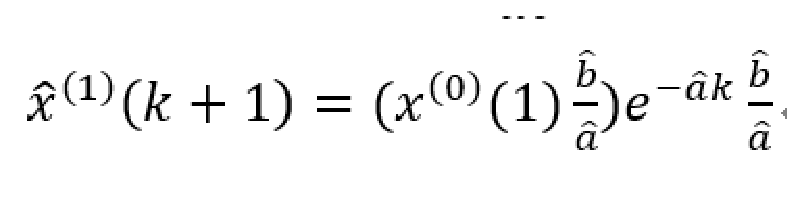
\includegraphics[width=0.6\textwidth]{fc.eps}
%				\caption{Whitening differential equation}
%				\label{fig:Pfc}
%			\end{minipage}
%		\end{figure}
	
	\begin{figure}[h]
		%\small
		\centering
		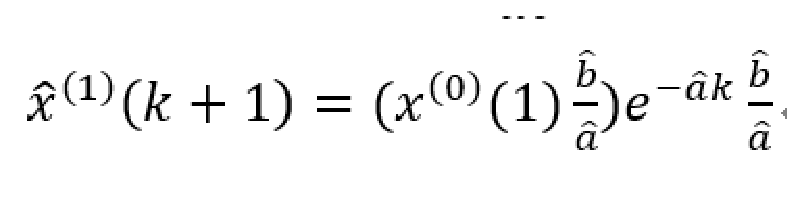
\includegraphics[width=5cm]{fc.eps}
		\caption{Whitening differential equation} \label{fig:fc}
	\end{figure}

		${x^{(0)}}$ is original sequence, ${x^{(1)}} $ is cumulative generating sequence. We can get the $y_{pred_{1,i}}$.
		
		\item[GM(2,1) Model] 
		\begin{equation}
		a^{(1)}x^{(0)}(k)+a_1 x^(0)(k)+a_2z^(1)(k)=b
		\end{equation}
		Whitening differential equation:
		$\frac{{{\partial ^2}{x^{(1)}}}}{{\partial {t^2}}} + {a_1}\frac{{{\partial ^{}}{x^{(1)}}}}{{\partial {t^{}}}} + {a_2}{x^{(1)}} = b$
		We can get the $y_{pred_{2,i}}$.
		
		\item[DGM(2,1) Model] 
		\begin{equation}
		{a^{(1)}}{x^{(0)}}(k) + {a_1}{x^{(0)}}(k) = b
		\end{equation}
		Whitening differential equation:$\frac{{{\partial ^2}{x^{(1)}}}}{{\partial {t^2}}} + a\frac{{{\partial ^{}}{x^{(1)}}}}{{\partial {t^{}}}} = b$. We can get the $y_{pred_{3,i}}$.
		
	\end{description}
	\item Use Combination Prediction Method to weight the predicted values of each model according to the errors of the three models.
	\begin{equation}
	err1=D1=\sum(y_{pred_{1,i}}-y_{1,i})^2 
	\end{equation}
	\begin{equation}
	err2=D2=\sum(y_{pred_{2,i}}-y_{2,i})^2  \\
\end{equation}
\begin{equation}
	err3=D3=\sum(y_{pred_{3,i}}-y_{3,i})^2  \\
\end{equation}
\begin{equation}
	{w_k} = \frac{{\frac{1}{{{D_k}}}}}{{\frac{1}{{{D_1}}} + \frac{1}{{{D_2}}} + \frac{1}{{{D_3}}}}}
	\end{equation}
	\item Compute prediction results under Combination Prediction Method
	\begin{equation}
	y_{pred_i}=\sum\limits_{k = 1}^3 {{w_k}{y_{pre{d_{k,i}}}}} 
	\end{equation}
\end{enumerate}


\paragraph{Solution Three:Linear Regression}
\par\noindent
\par\noindent
From the point of view of the employment situation of Chinese students and the overall situation of China, establish the regression equation , which includes the total number of posts per year (y) and the first employment number of university graduates (ugea), the same enrollment number of universities (ugc), the gross domestic product (gdp), the total urban population (eyua), the total rural population (etaa) at the end of the year and natural growth rate of population in China. The regression equation can be expressed by the following equation:
\begin{equation}
y=\beta_0+\beta_1ugea+\beta_2ugc+\beta3gdp+\beta_4eyua+\beta_5etaa+\beta_6g+u
\end{equation}
	After the regression equation of 2015-2018 is obtained, the data of a, b, gdp, c, d, e in the next three years are obtained through the grey prediction GM (1,1) model, and then bring them into the regression equation again to get the total number of posts in the next three years - the value of potential talent demand.

The flow chart for whole solutions of Problem Two: figure \ref{fig:Plct2}.
\begin{figure}[h]
	%\small
	\centering
	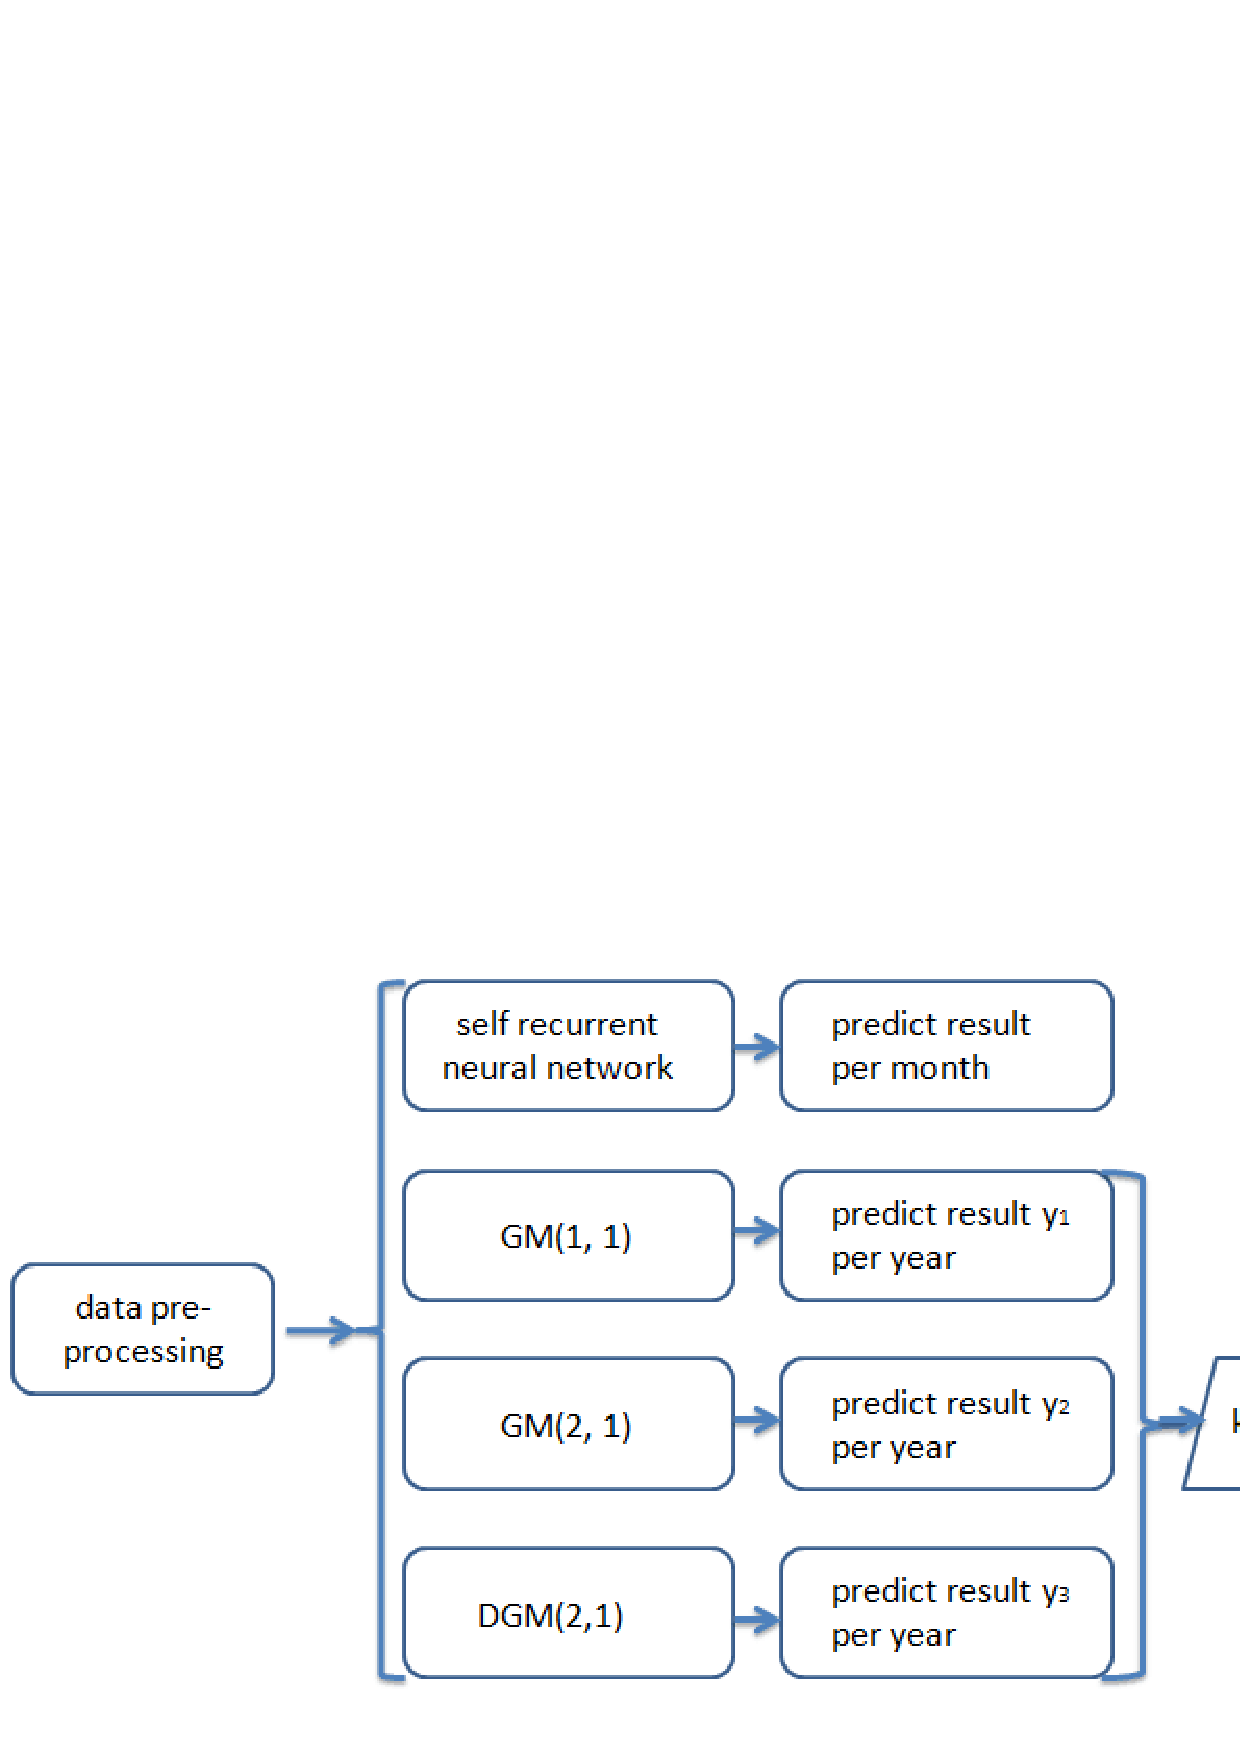
\includegraphics[width=12cm]{lct2.png}
	\caption{flow chart in Problem 2} \label{fig:Plct2}
\end{figure}

\subsubsection{Results Analysis}
Clearly, this problem is based on the model of Problem One. At the beginning, let's analysis from the perspective of ``job market of A-City''.\\
 By using autoregressive\_artificial\_neutal\_nets, we get a basic prediction result of next three years in every industry: The abscissa is time (each time point is three months, which means a quarter, for example, time point 1 is the first quarter of 2019, time point 5 is the first quarter of 2020), the ordinate is the job supply of A-City (unit: person). The results of the model are shown in the figure ~\ref{fig:P2.1} to figure \ref{fig:P2.3} (with Art/graphics/Animation design as an example and other figures please see the supporting materials).

%!PS-Adobe-3.0 EPSF-3.0 
%BoundingBox: 5 5 105 105
%
%\begin{figure}[h]
%	%\small
%	\centering
%	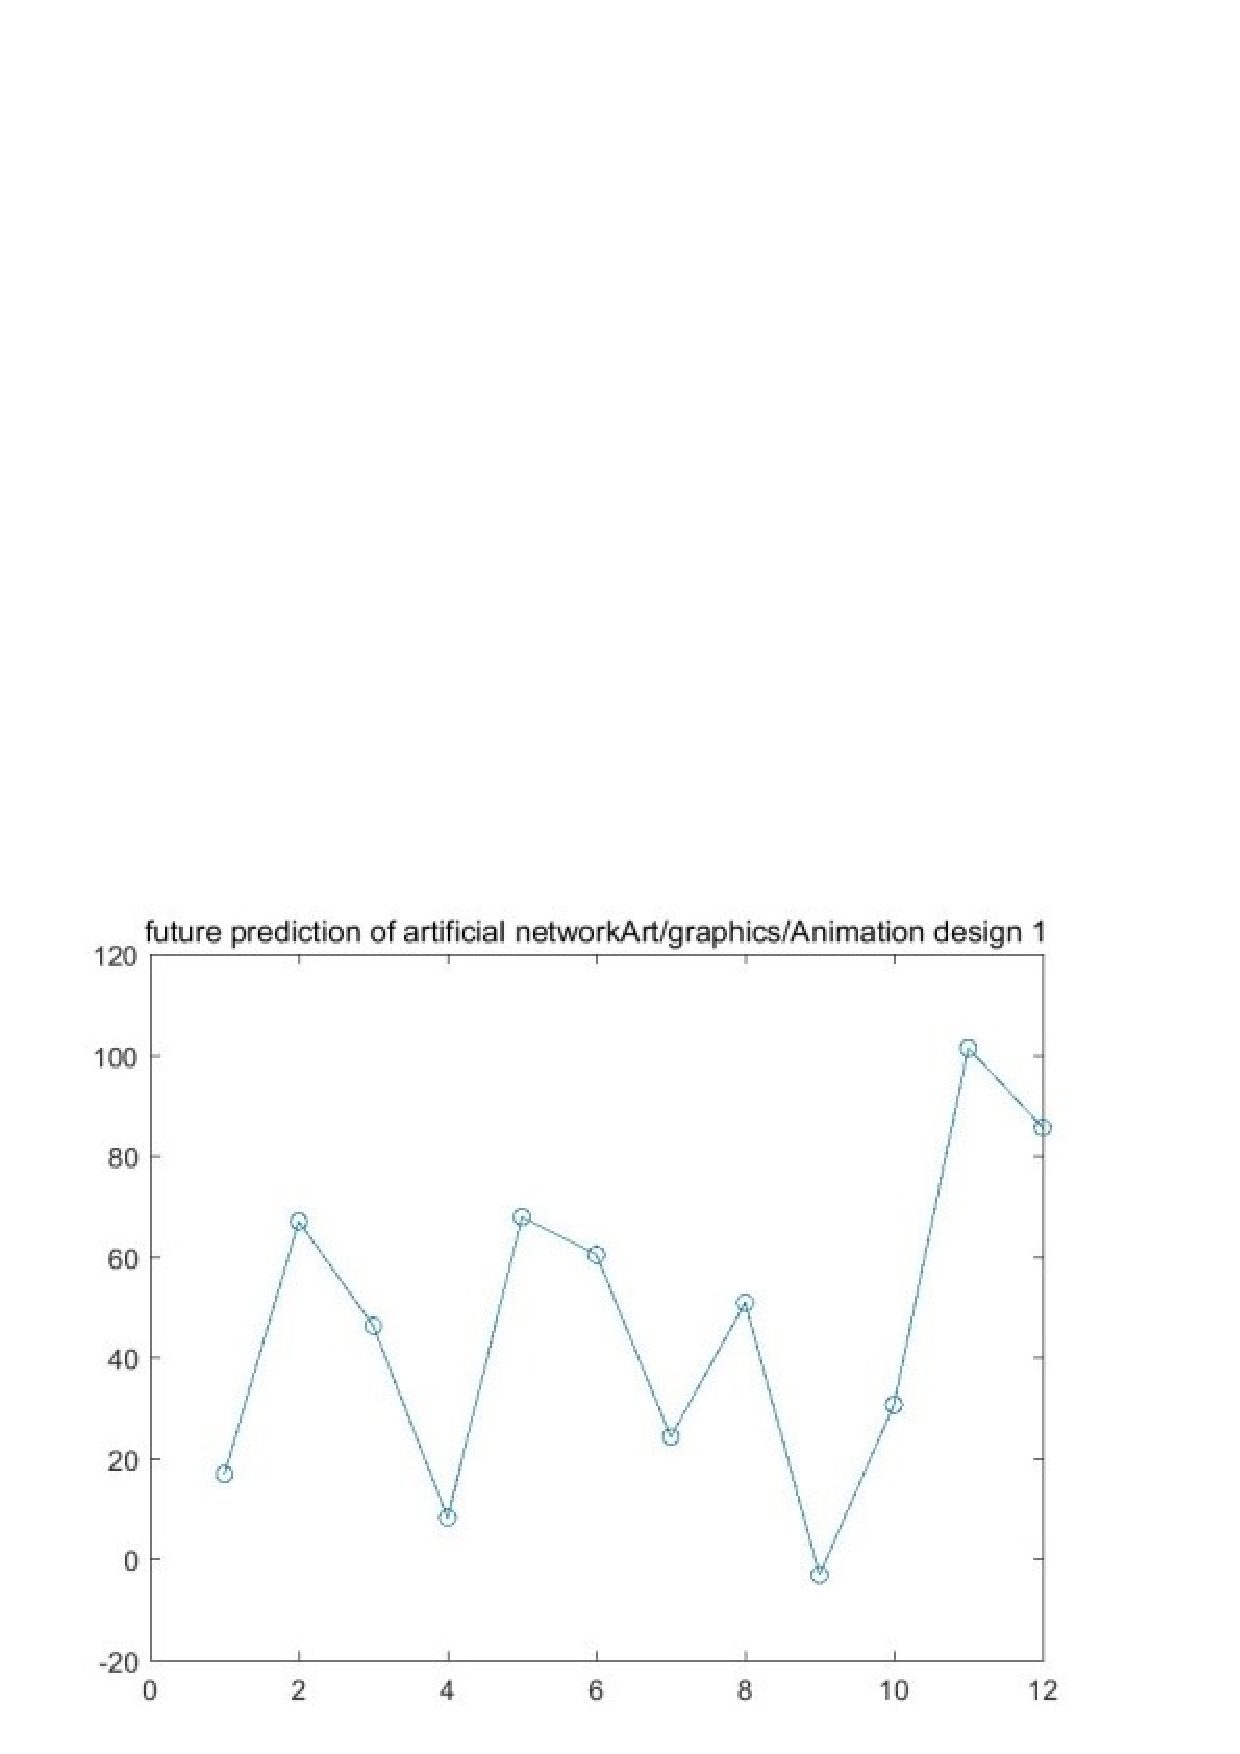
\includegraphics[width=1cm]{2.1.jpg}
%	\caption{low education} \label{fig:P2.1}
%\end{figure}

%\begin{figure}     \centering     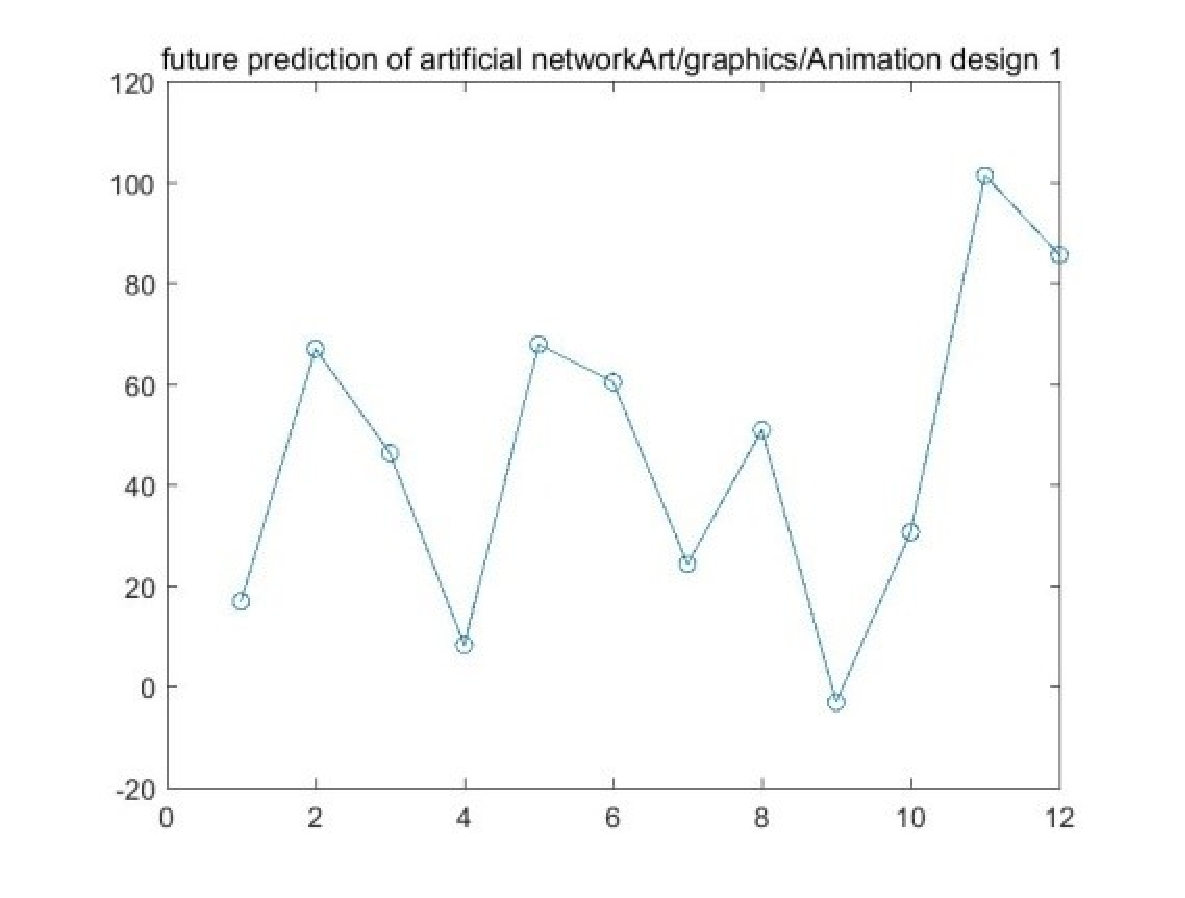
\includegraphics[totalheight=2.5in]{2.1.eps}     \caption{low education}     \label{fig:test} 
%\end{figure}
%
%
%\begin{figure}     \centering     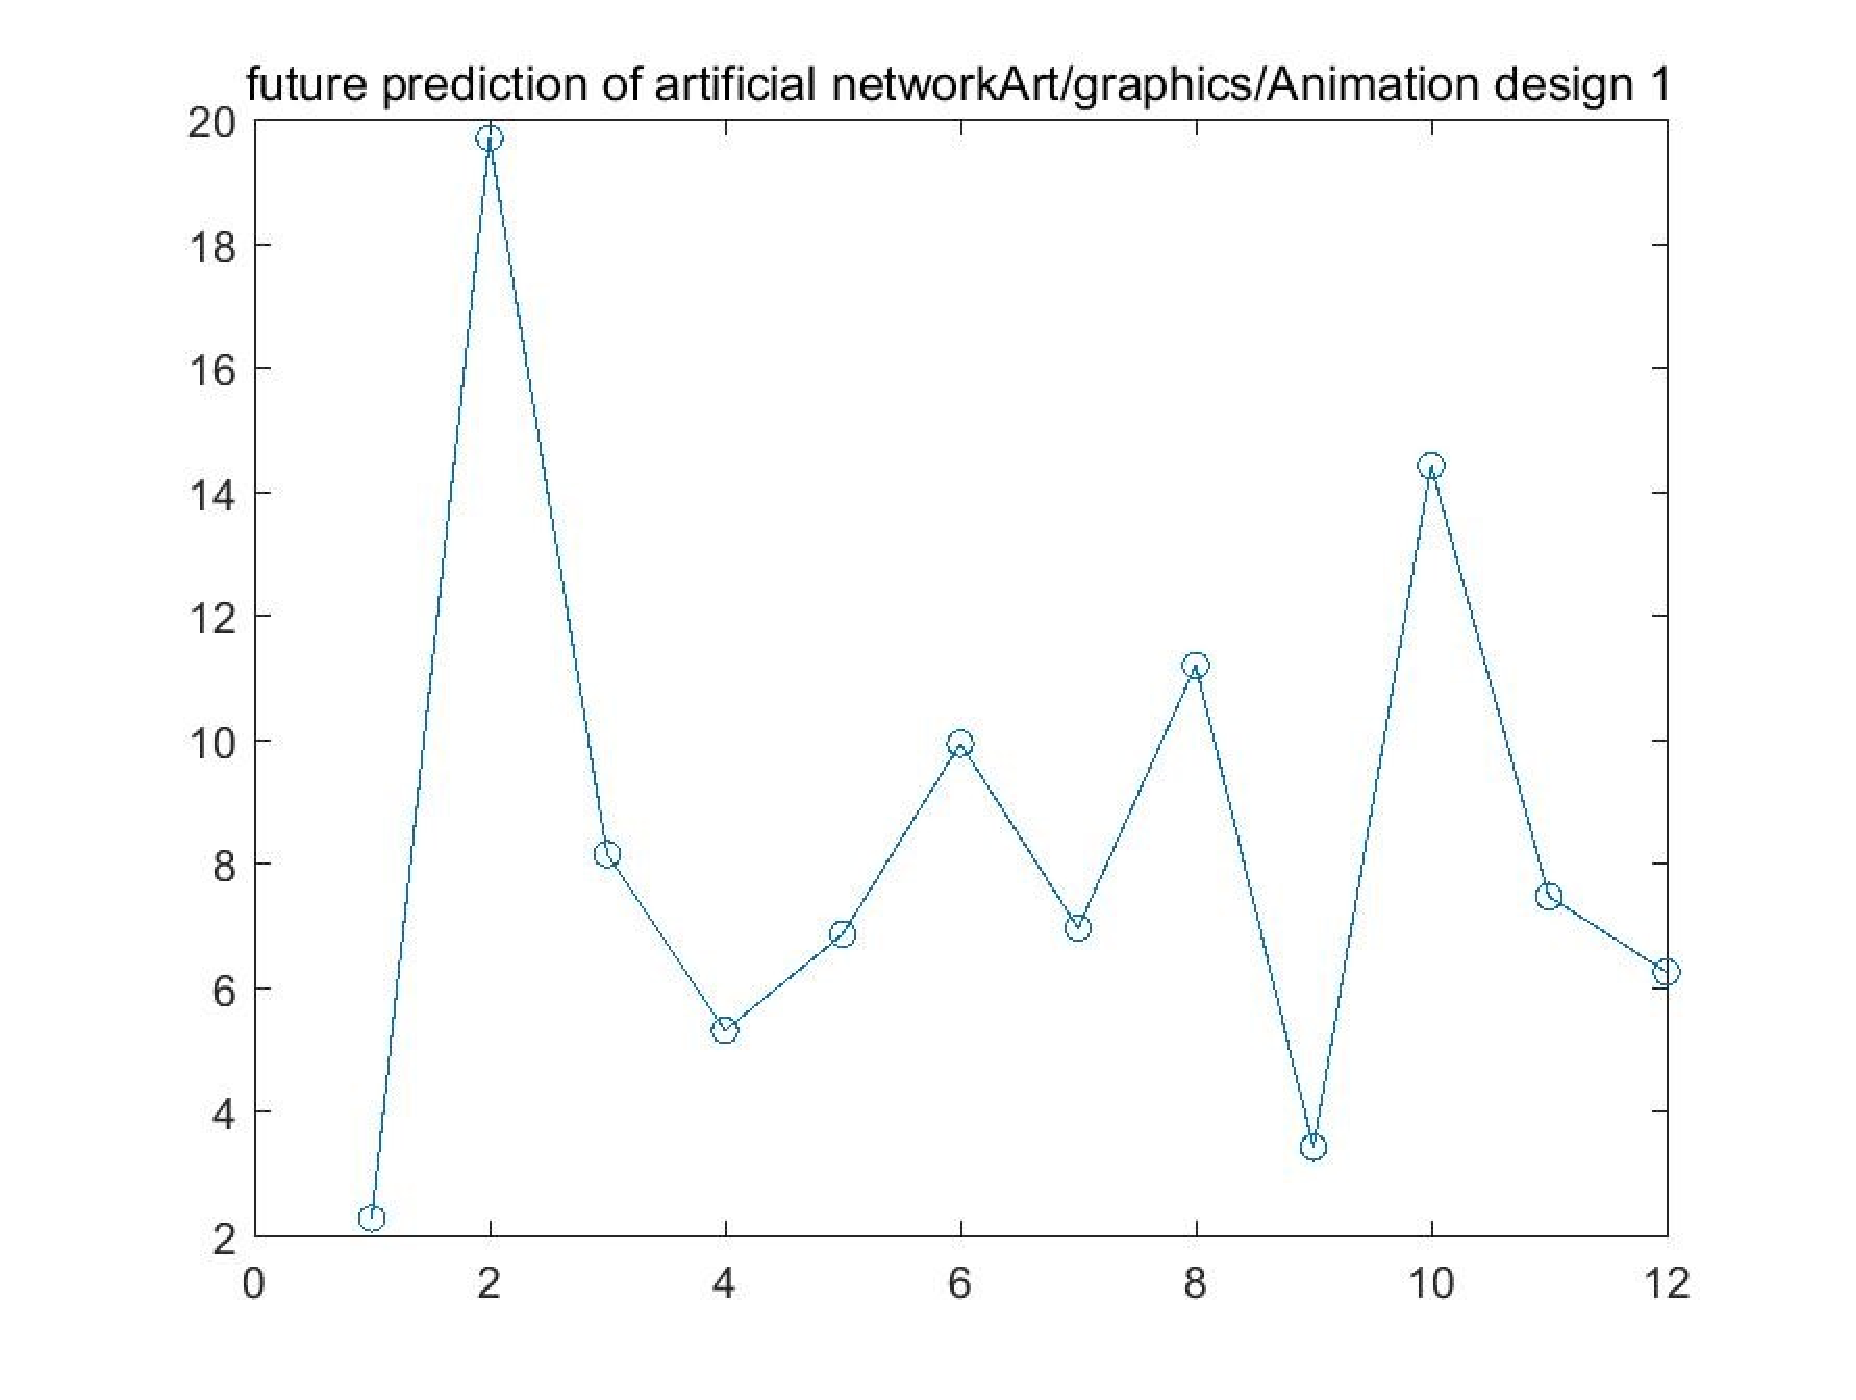
\includegraphics[totalheight=2.5in]{2.2.eps}     \caption{low education}     \label{fig:test} 
%\end{figure}
%
%\begin{figure}     \centering     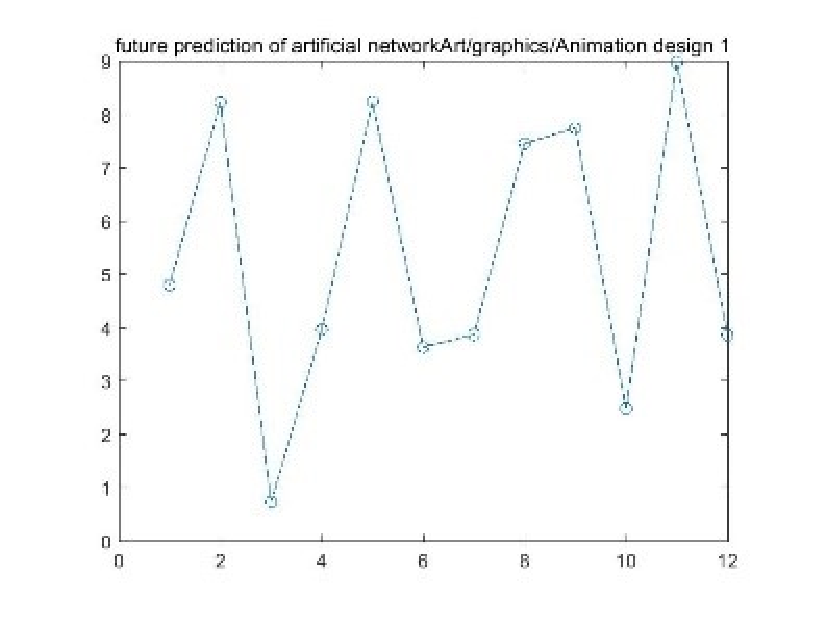
\includegraphics[totalheight=2.5in]{2.3.eps}     \caption{low education}     \label{fig:test} 
%\end{figure}

\begin{figure}[h]
	\begin{minipage}[h]{0.31\linewidth}
		\centering
		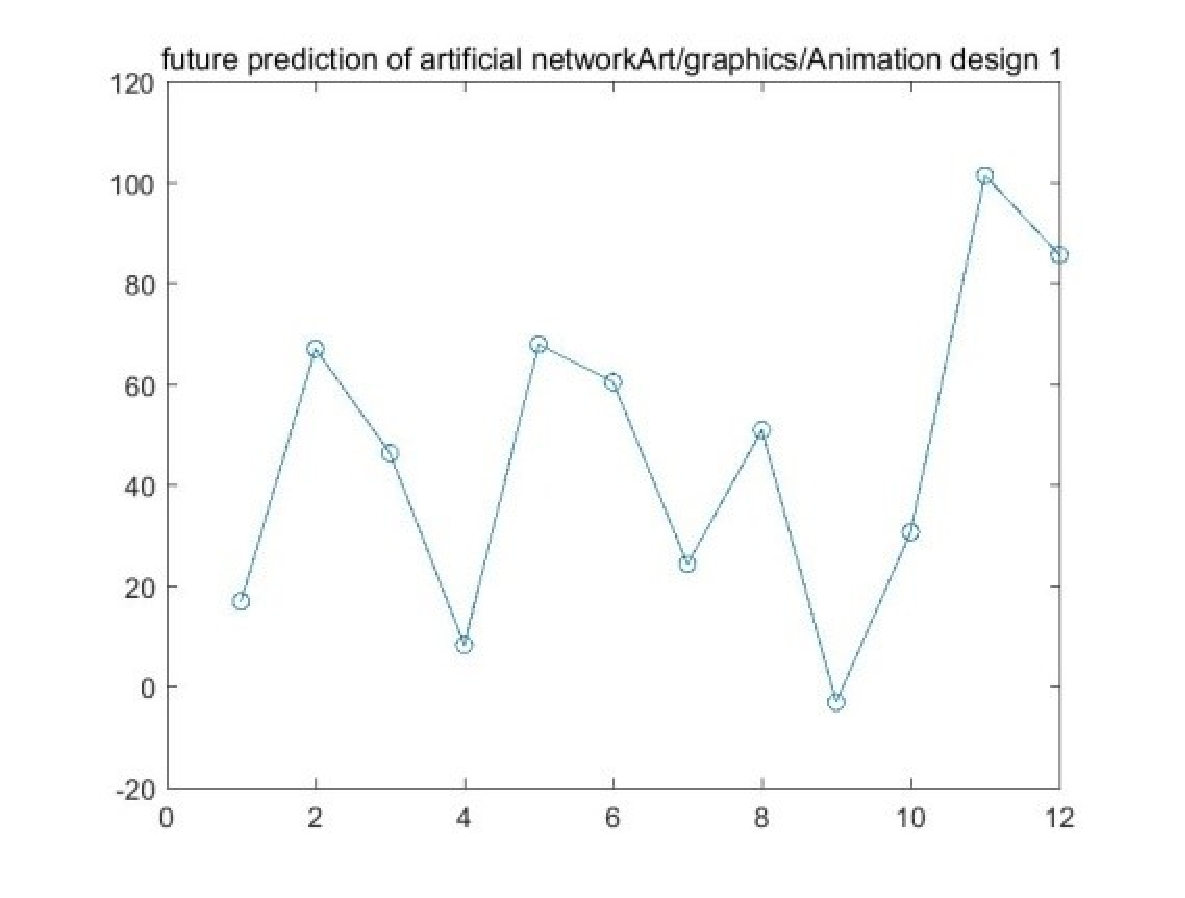
\includegraphics[width=1\textwidth]{2.1.eps}
		\caption{low education}
		\label{fig:P2.1}
	\end{minipage}
	\begin{minipage}[h]{0.31\linewidth}
		\centering
		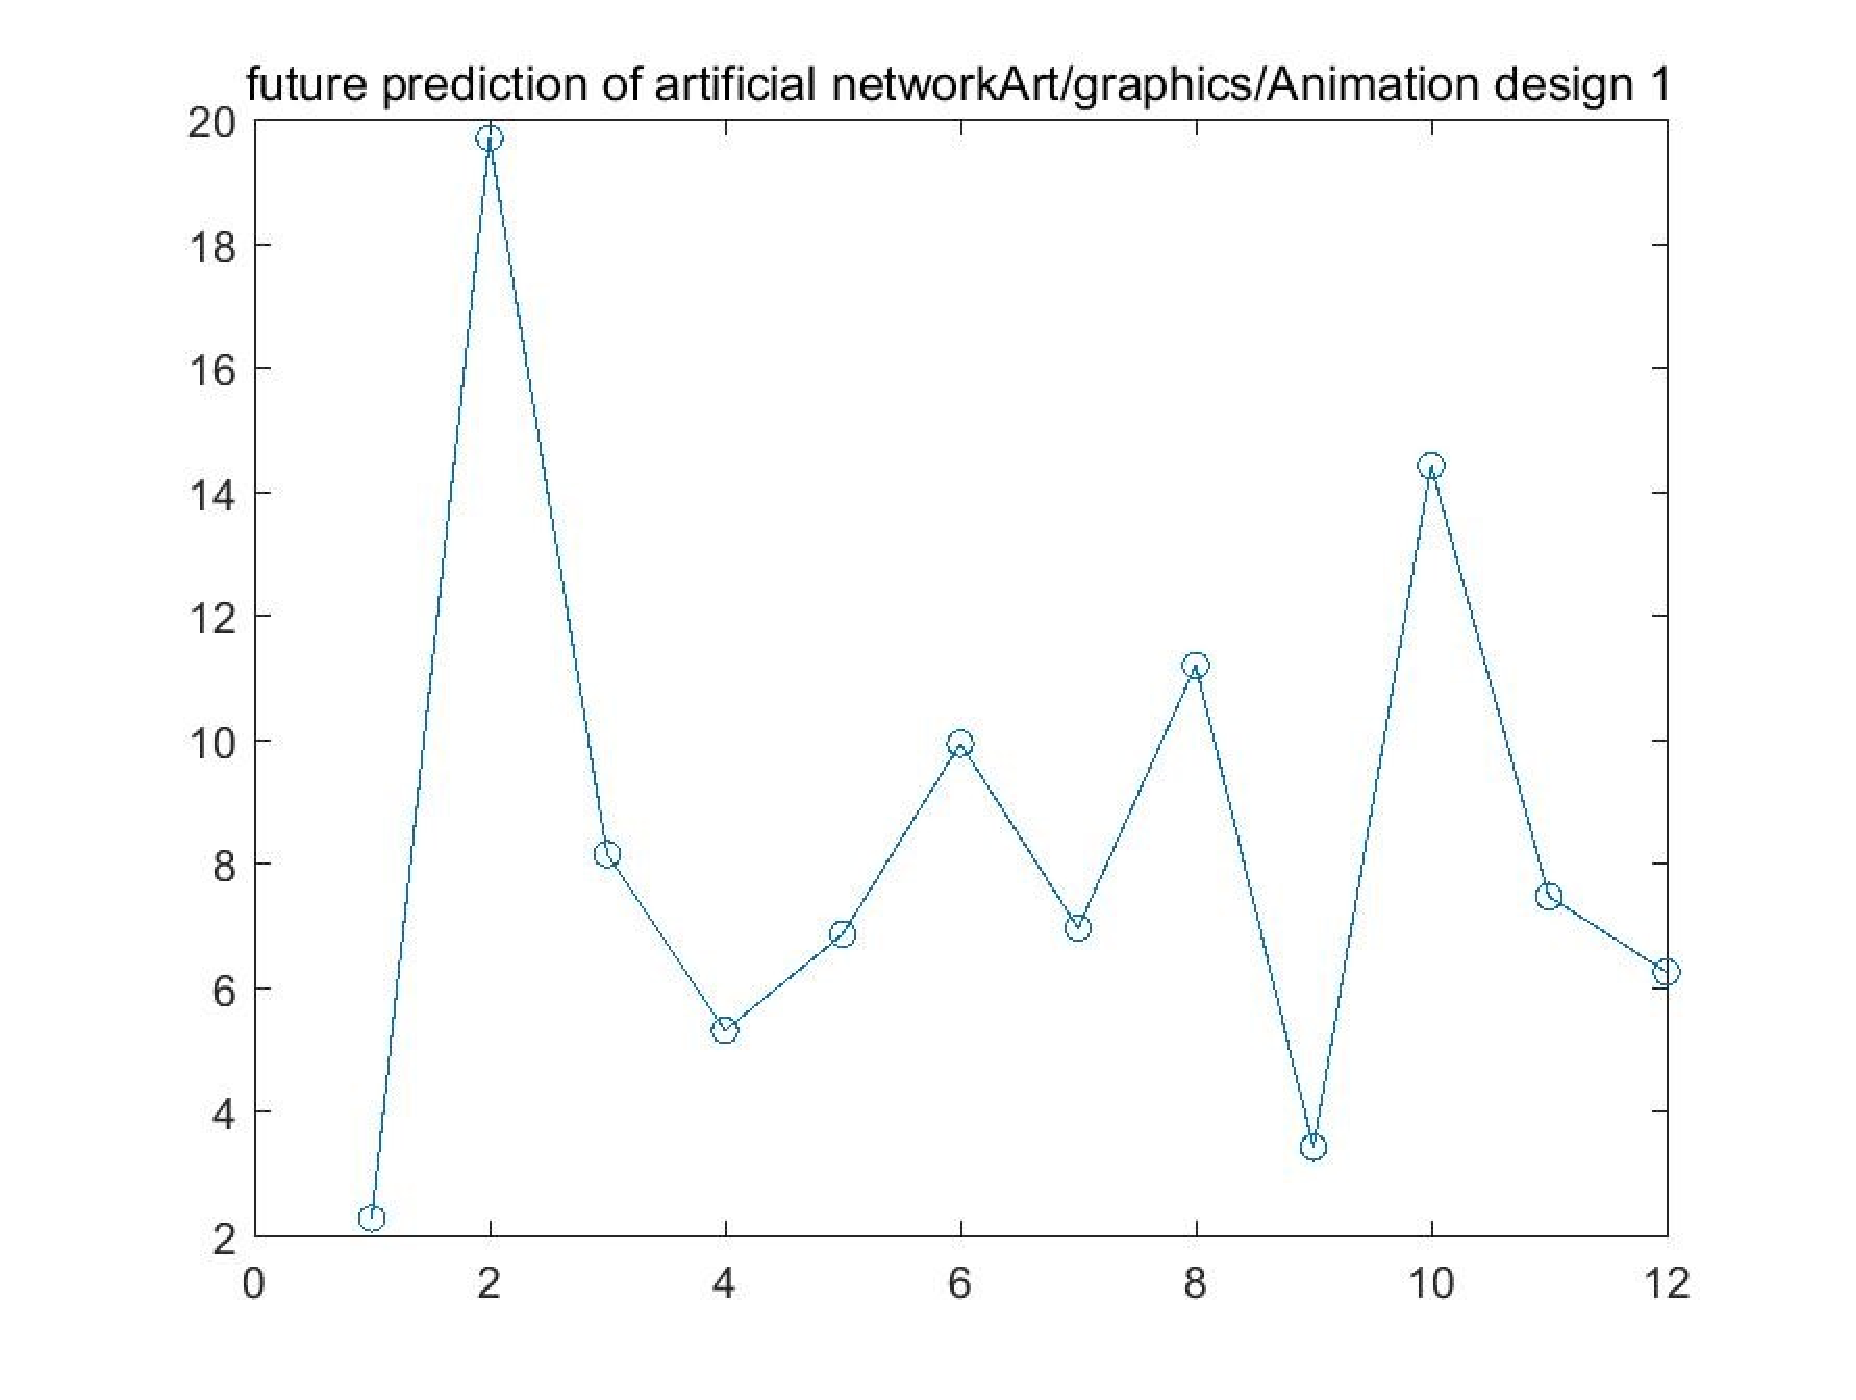
\includegraphics[width=1\textwidth]{2.2.eps}
		\caption{medium education}
		\label{fig:P2.2}
	\end{minipage}
	\begin{minipage}[h]{0.31\linewidth}
		\centering
		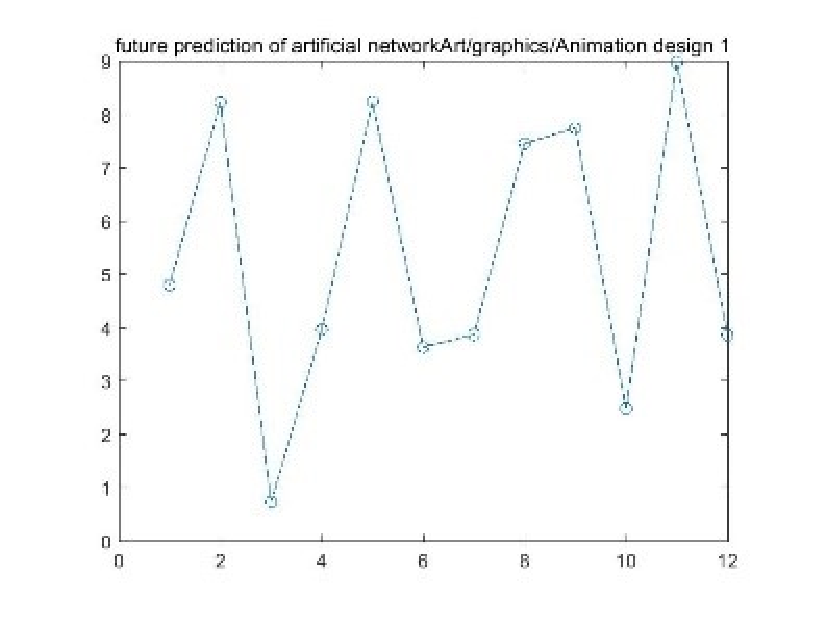
\includegraphics[width=1\textwidth]{2.3.eps}
		\caption{Unlimited}
		\label{fig:P2.3}
	\end{minipage}
\end{figure}

%\begin{figure}
%	\begin{subfigure}[b]{.5\linewidth}
%		\centering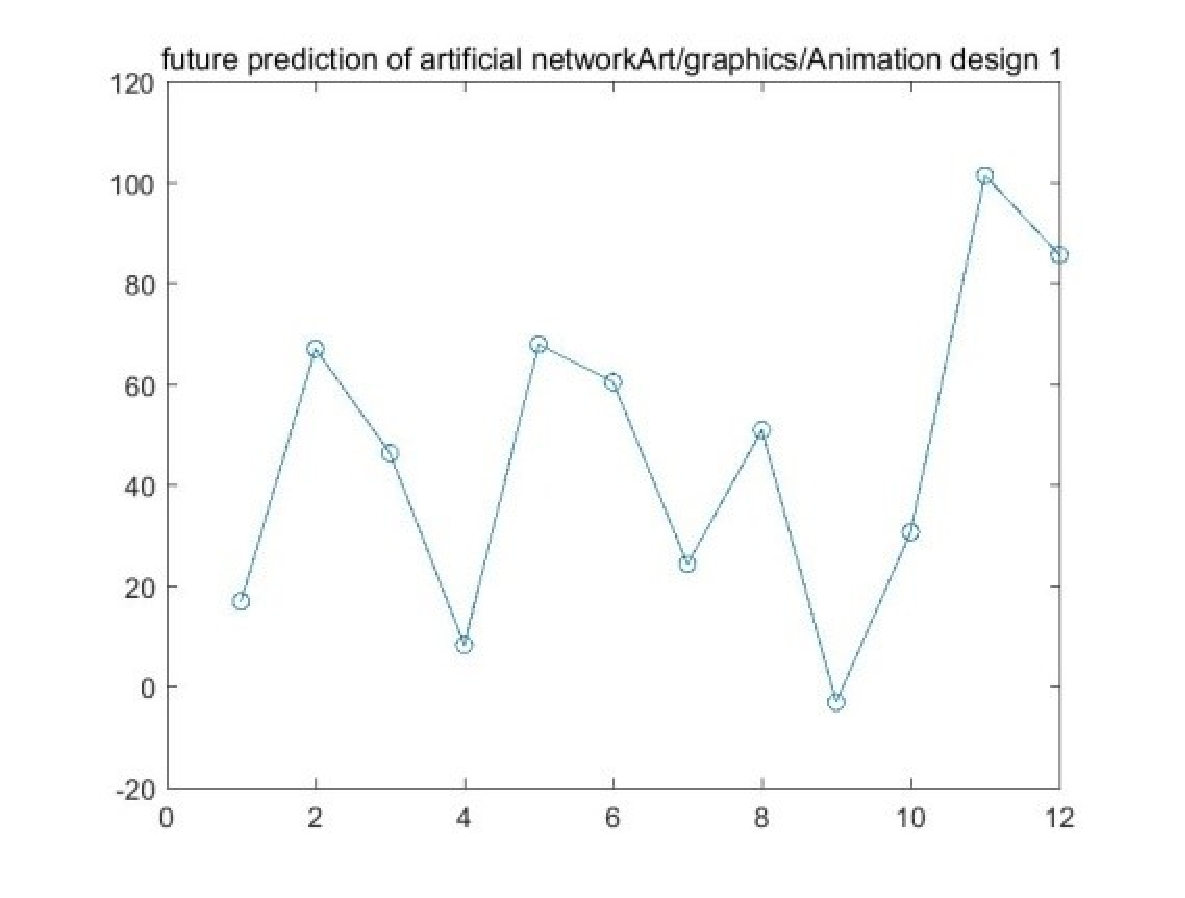
\includegraphics[width=0.8\textwidth]{2.1.eps}
%		\caption{A subfigure}\label{fig:2a}
%	\end{subfigure}%
%	\begin{subfigure}[b]{.5\linewidth}
%		\centering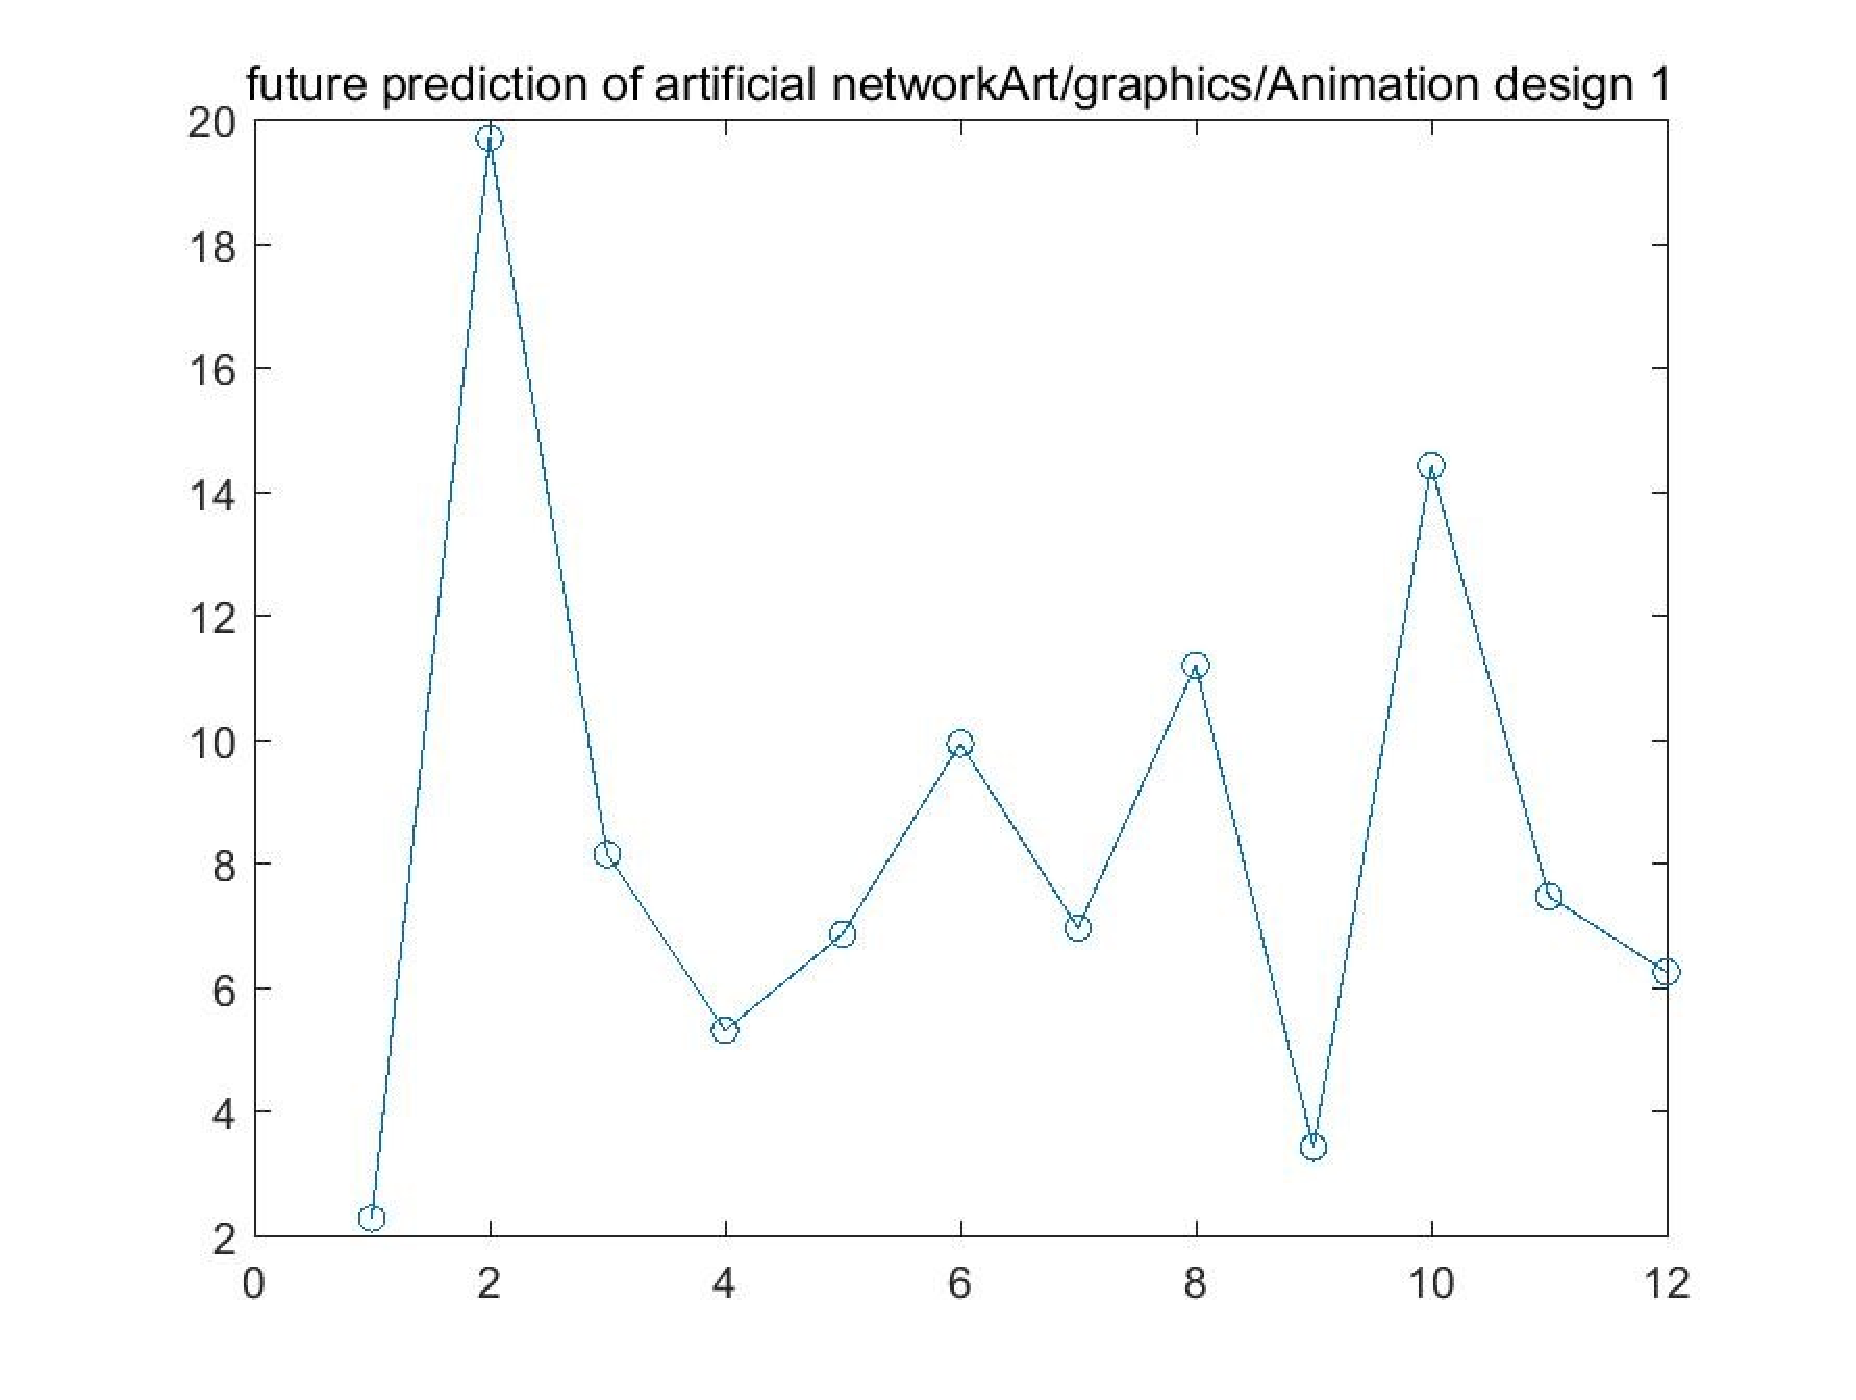
\includegraphics[width=0.8\textwidth]{2.2.eps}
%		\captionsetup{skip=0pt}
%		\caption{Another subfigure}\label{fig:2b}
%	\end{subfigure}
%	\caption{A figure}\label{fig:2}
%\end{figure}


\par\noindent
Figure 1 is the sum of the number of jobs offered by various industries which require low education(Junior middle school、Senior middle school 、Technical secondary school). Figure 2 means medium education requirements(Junior college、Bachelor's degree、Master's degree). Figure 3 means unlimited educational requirement. Due to the over-small non-zero data samples which require Master’s degree、Doctor’s degree and MBA background, the error of the predicted results is too large, so these data are discarded.

\par\noindent
The results based on three kinds of gray prediction are shown in the following figure \ref{fig:P2.4} to \ref{fig:P2.9} (the order of display is the same as above).

\begin{figure}[h]
	\begin{minipage}[h]{0.31\linewidth}
		\centering
		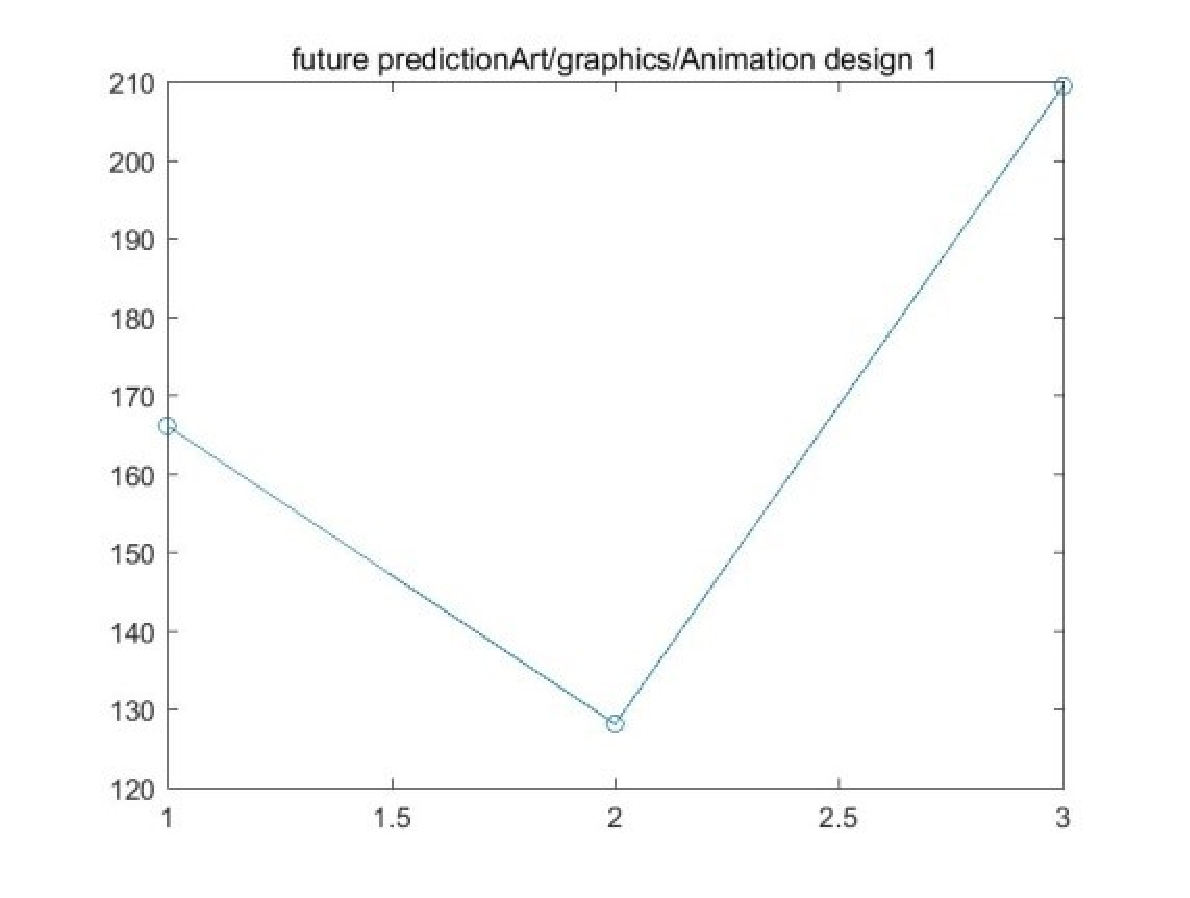
\includegraphics[width=1\textwidth]{2.4.eps}
		\caption{low education}
		\label{fig:P2.4}
	\end{minipage}
	\begin{minipage}[h]{0.31\linewidth}
		\centering
		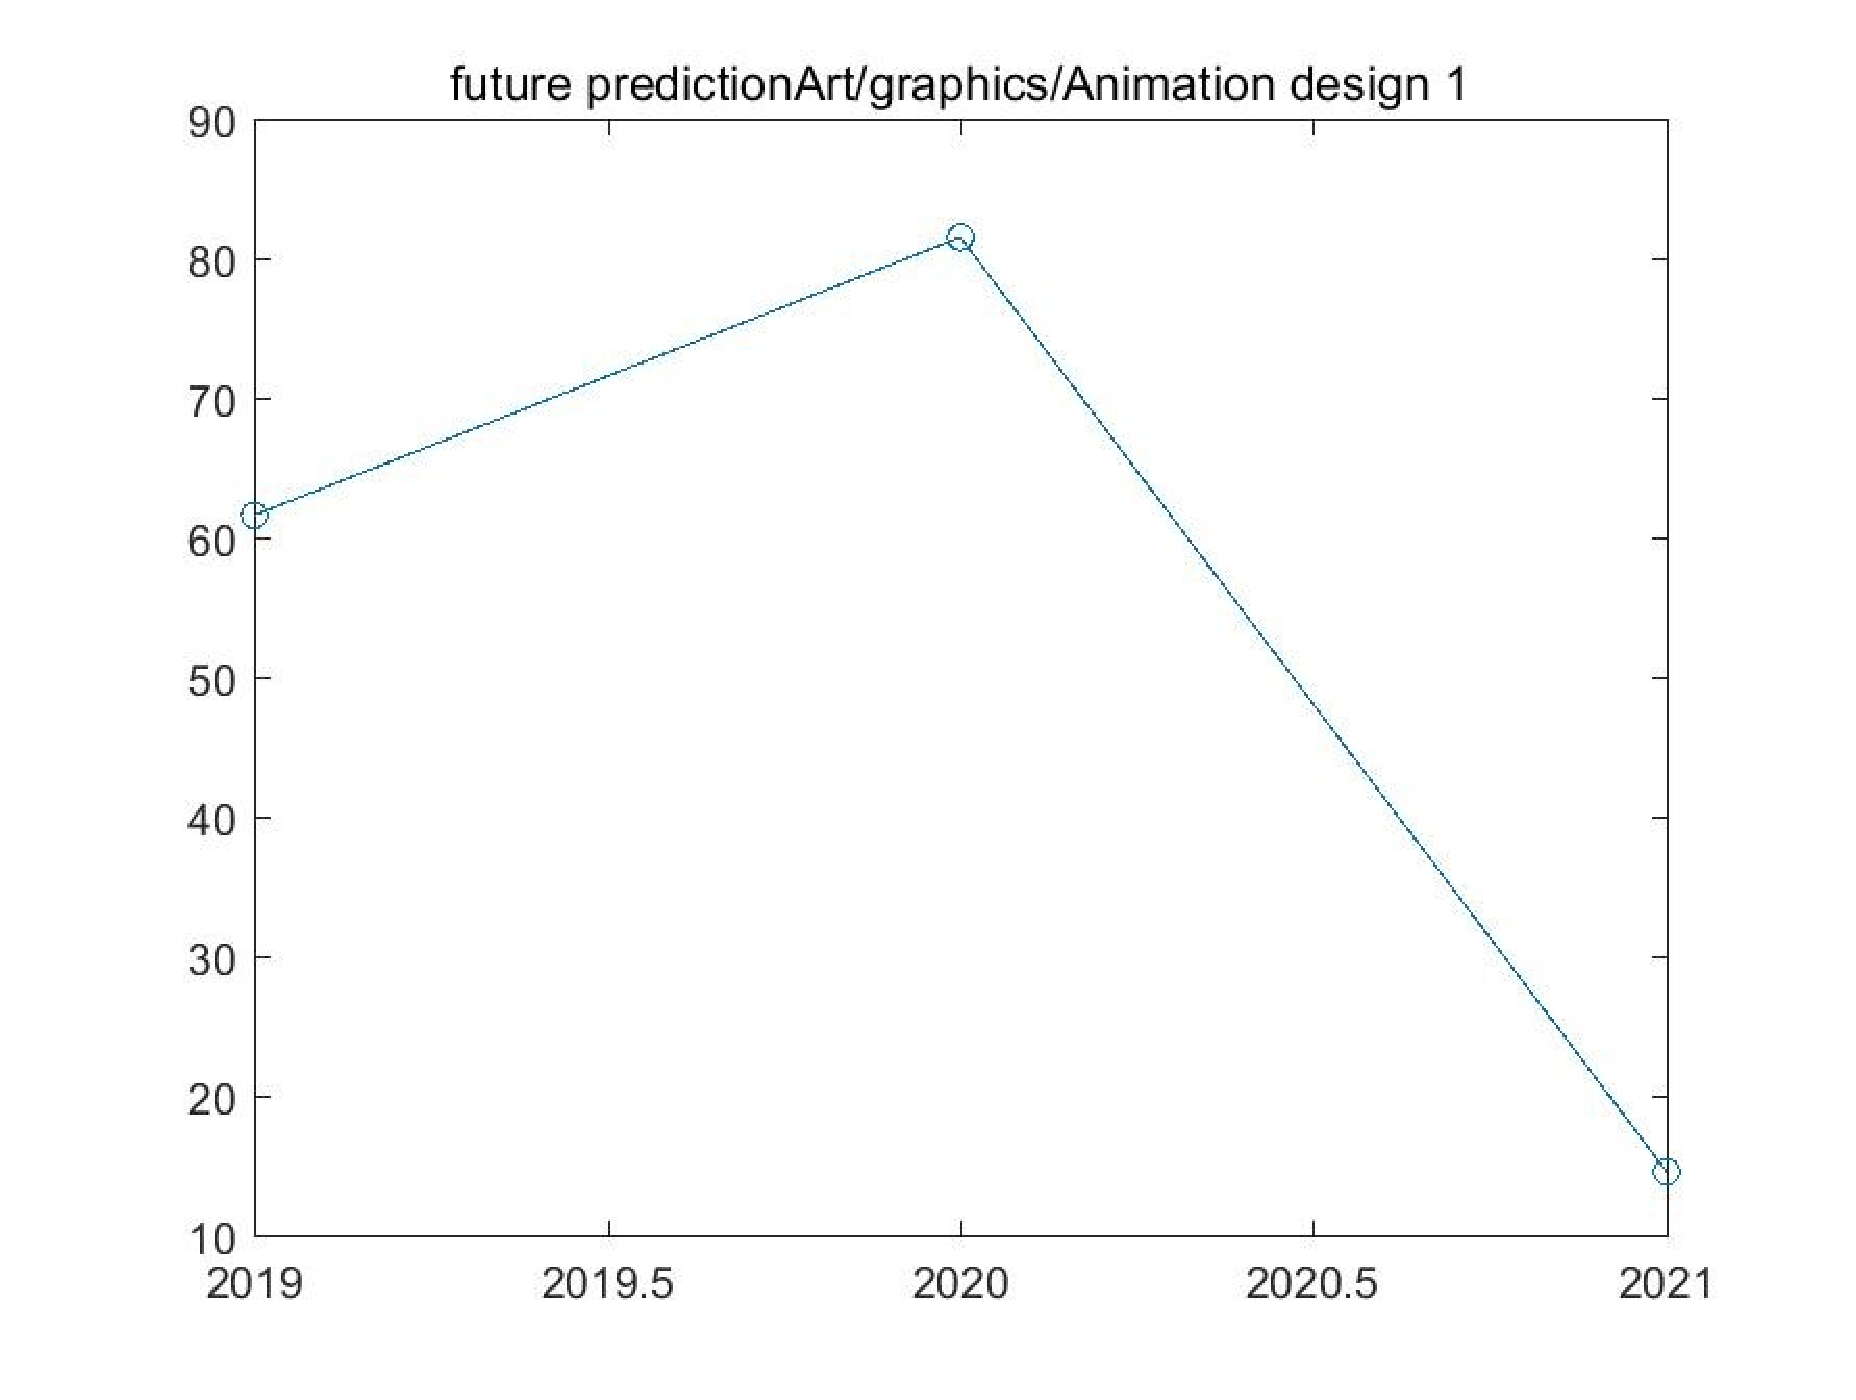
\includegraphics[width=1\textwidth]{2.5.eps}
		\caption{medium education}
		\label{fig:P2.5}
	\end{minipage}
	\begin{minipage}[h]{0.31\linewidth}
		\centering
		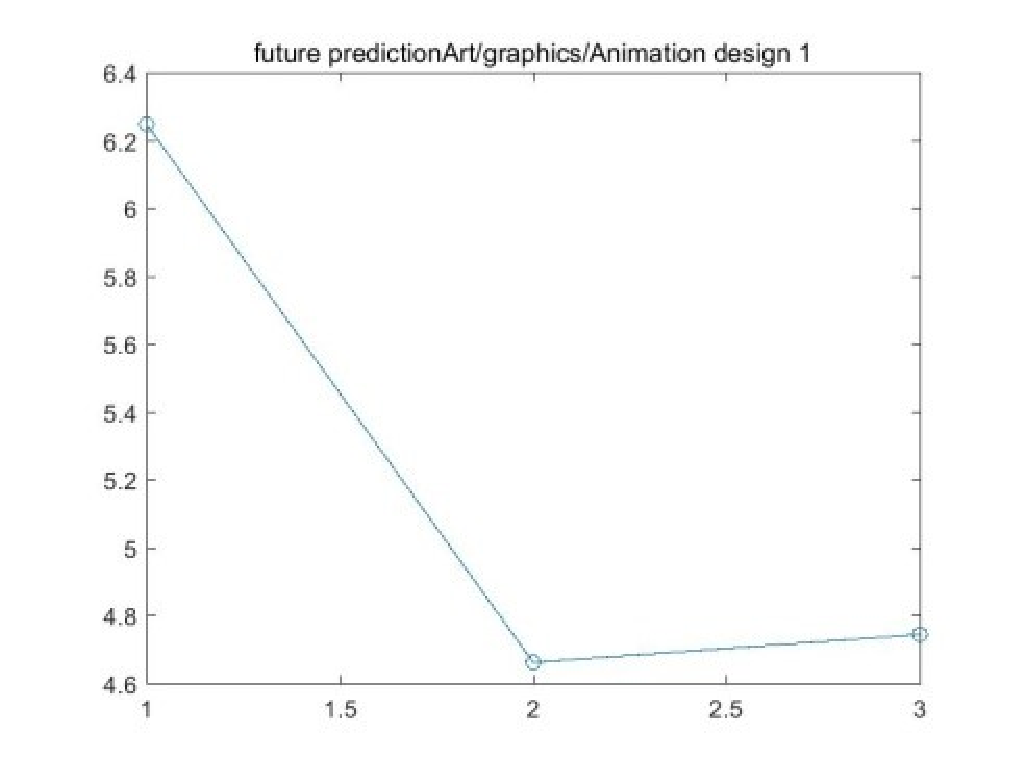
\includegraphics[width=1\textwidth]{2.6.eps}
		\caption{Unlimited}
		\label{fig:P2.6}
	\end{minipage}
\end{figure}

\begin{figure}[h]
	\begin{minipage}[h]{0.31\linewidth}
		\centering
		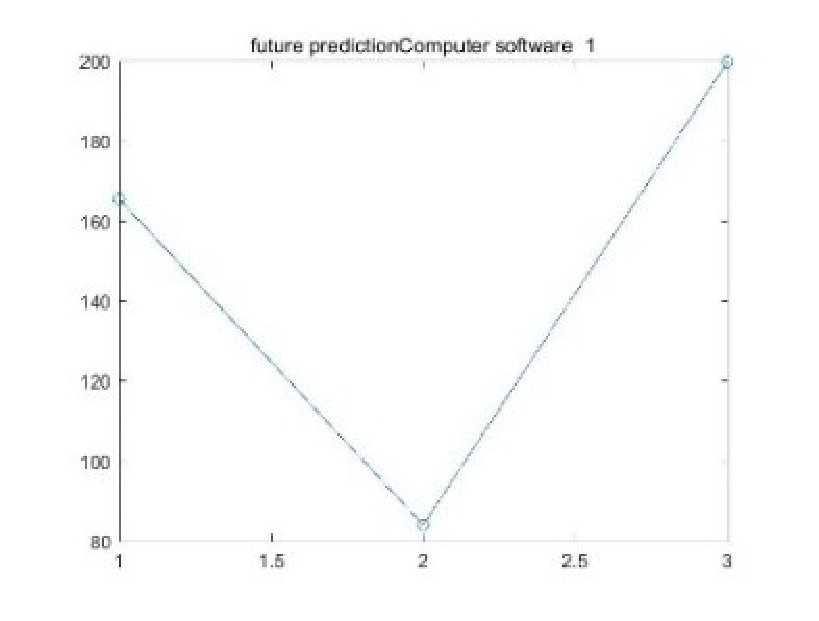
\includegraphics[width=1\textwidth]{2.7.eps}
		\caption{low education}
		\label{fig:P2.7}
	\end{minipage}
	\begin{minipage}[h]{0.31\linewidth}
		\centering
		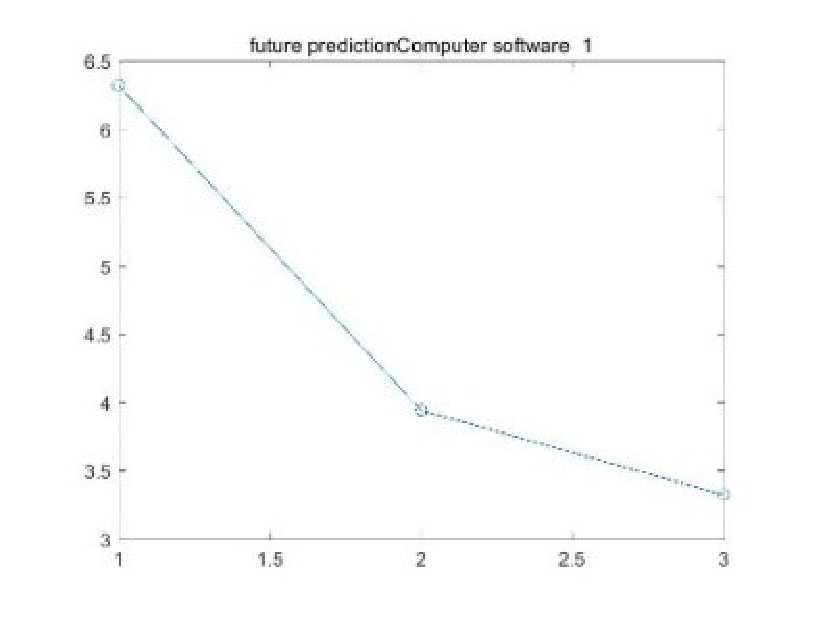
\includegraphics[width=1\textwidth]{2.8.eps}
		\caption{medium education}
		\label{fig:P2.8}
	\end{minipage}
	\begin{minipage}[h]{0.31\linewidth}
		\centering
		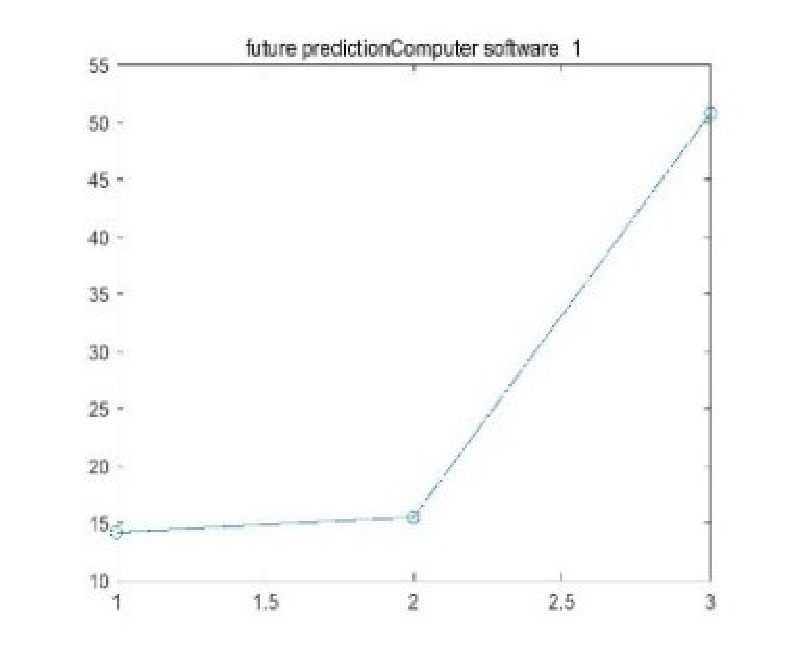
\includegraphics[width=1\textwidth]{2.9.eps}
		\caption{Unlimited}
		\label{fig:P2.9}
	\end{minipage}
\end{figure}

\par\noindent
Based on the grey forecasting method, we can get the talent demand forecasting pictures of all industries in the next three years in the attached data set. We take art departments ( figure\ref{fig:P2.1} to figure \ref{fig:P2.3}) and computer departments ( figure\ref{fig:P2.4} to figure \ref{fig:P2.6}) as representatives to analyze the inspiration of graphics. We can see that the requirements for academic qualifications of art departments are relatively low, which is also in line with our common senses. Moreover, the demand for talents in art departments is greatly influenced by the market. Compared with other traditional industries and the high-tech industries which are developing rapidly, a mature demand system for talents has not yet been formed. Therefore, we did not get a stable trend of prediction results. However, the computer industry has significantly improved the requirements for academic qualifications along with a higher threshold for entry. With the development of artificial intelligence, the demand of computer departments for highly educated personnel will grow. Of course, this is just the tip of the iceberg, for detailed results of other industries please see the supporting materials.

\par\noindent
According to the results obtained from gray level prediction in three years, sum over the number of people required for all academic qualifications in each industry, and then get the results of all jobs provided by each industry in every year which are figure \ref{fig:P2.10} to figure \ref{fig:P2.12}(from 2019 to 2021).
\begin{figure}[h]
	\begin{minipage}[h]{0.31\linewidth}
		\centering
		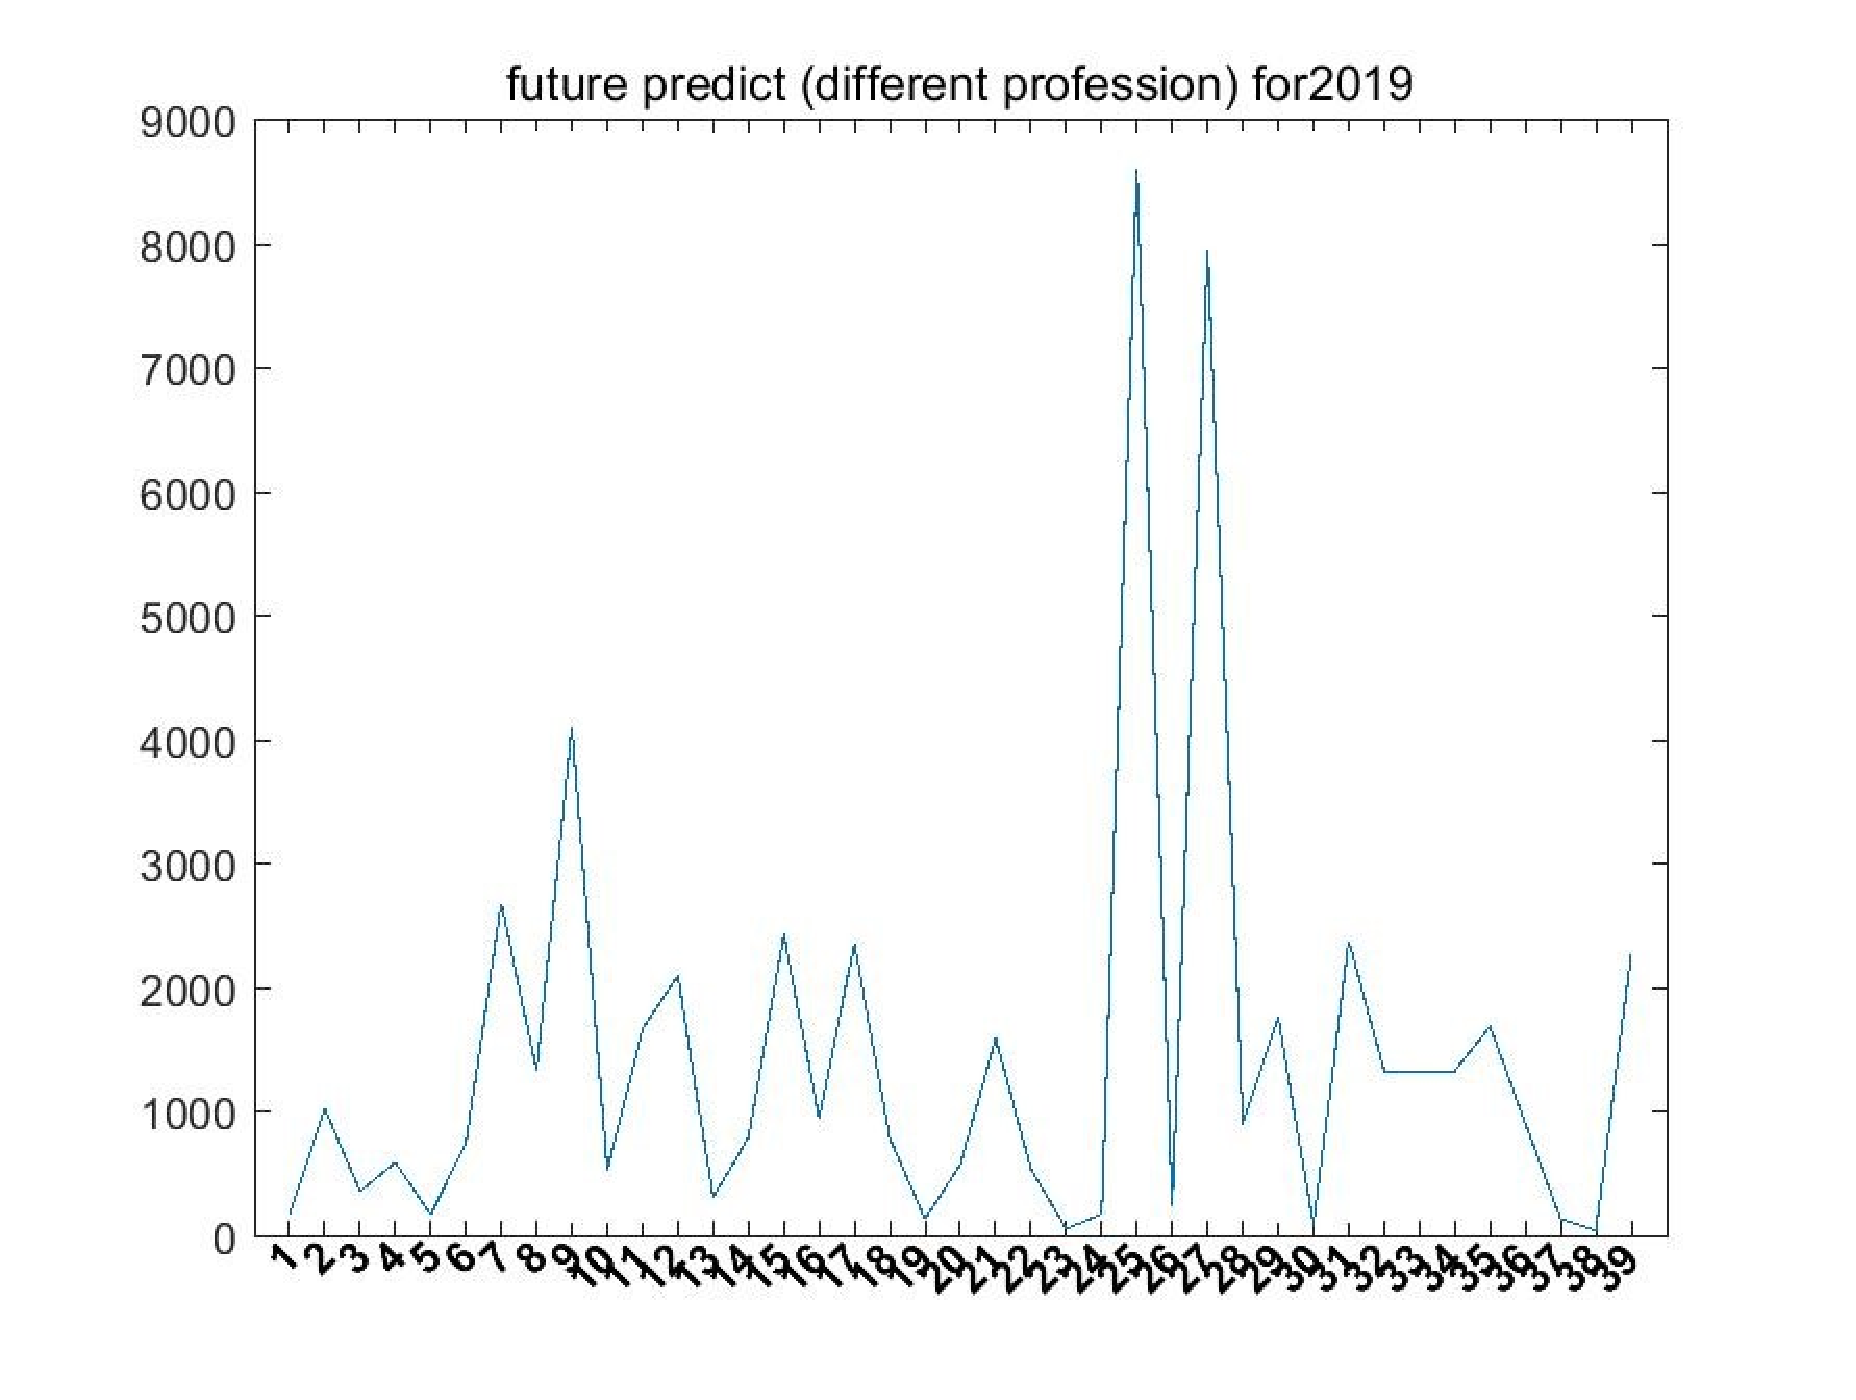
\includegraphics[width=1\textwidth]{2.10.eps}
		\caption{all posts in 2019}
		\label{fig:P2.10}
	\end{minipage}
	\begin{minipage}[h]{0.31\linewidth}
		\centering
		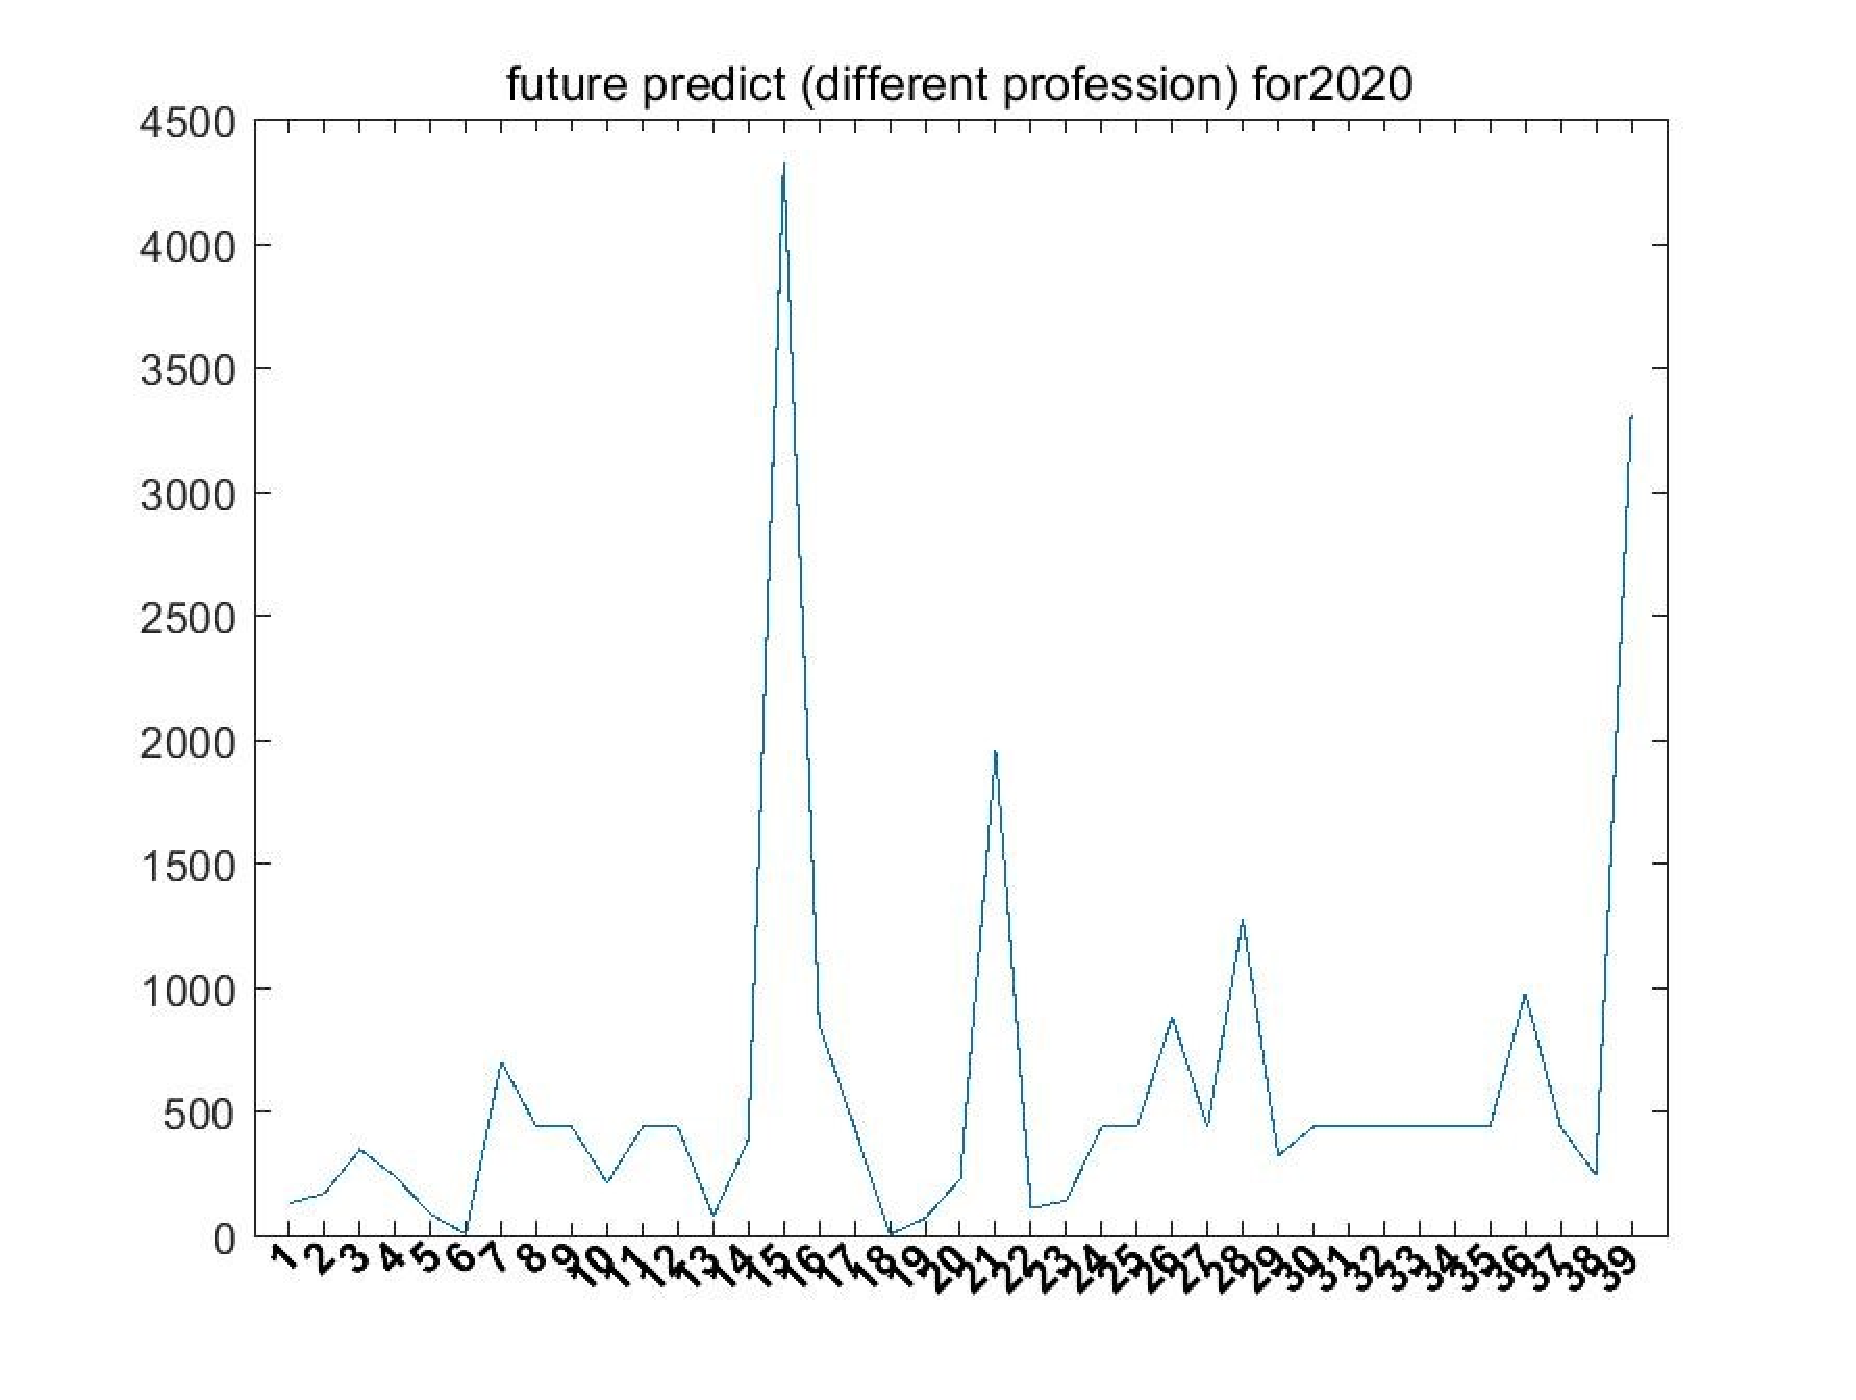
\includegraphics[width=1\textwidth]{2.11.eps}
		\caption{all posts in 2020}
		\label{fig:P2.11}
	\end{minipage}
	\begin{minipage}[h]{0.31\linewidth}
		\centering
		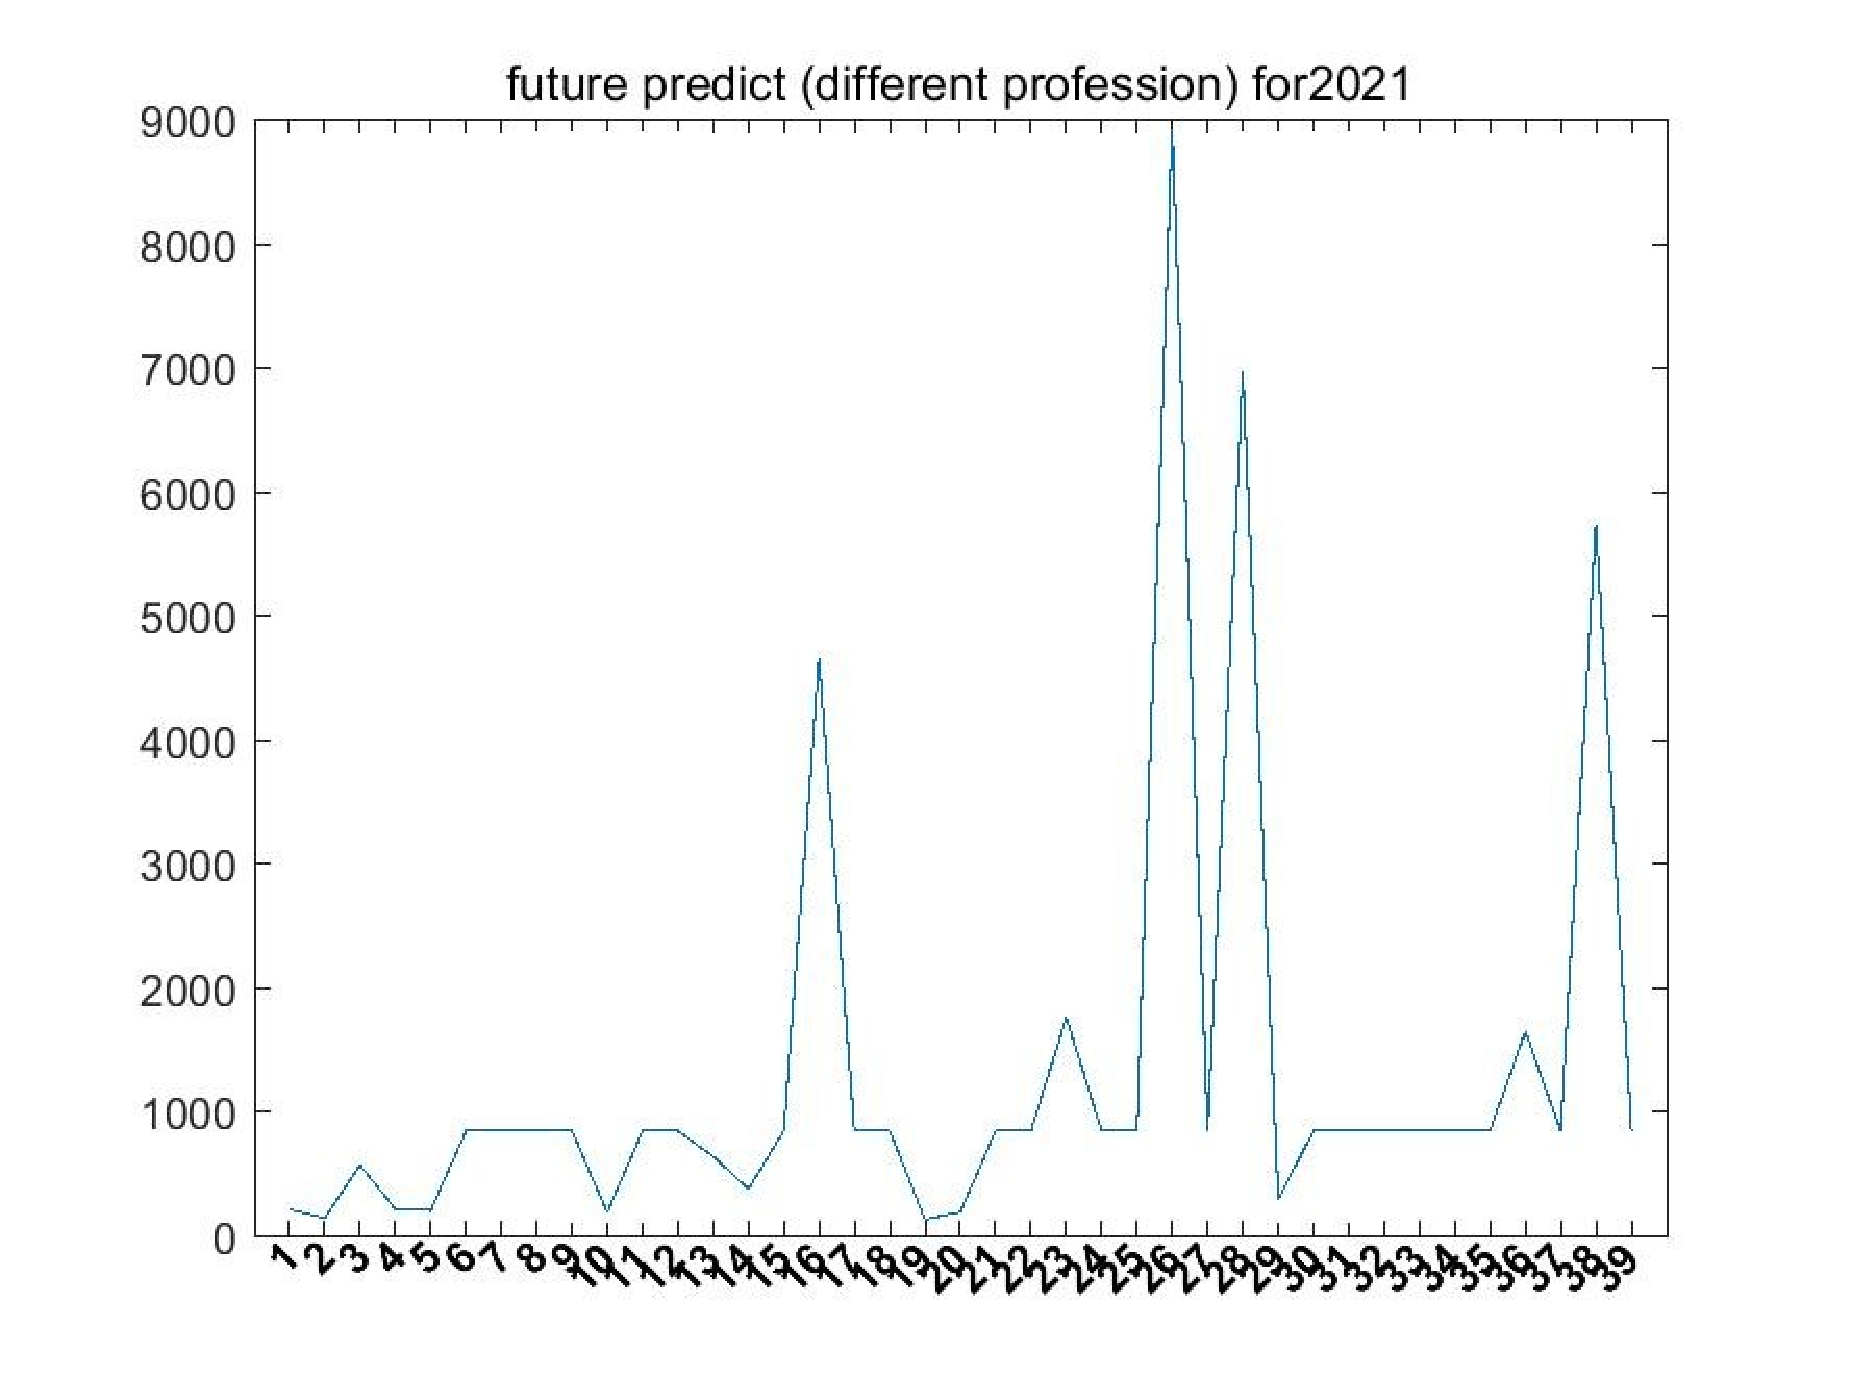
\includegraphics[width=1\textwidth]{2.12.eps}
		\caption{all posts in 2021}
		\label{fig:P2.12}
	\end{minipage}
\end{figure}
For detailed information of label 1~39, please see supporting material.
\par\noindent
In the next three years, the demand for talents in the financial industry, logistics industry and computer industry will be at a high level. However, the demand for talents in industries such as art and advertising will not change greatly, and it is always at a low level.According to the results, in the next three years, the demand for talents in mainstream industries has been at a high level. The demand for talent in some faster-growing industries is increasing year by year. The demand for talents in some immature departments has been at a low level.
\par\noindent
From the perspective of the employment situation of college students and China's national conditions, the results of solving the regression model are as follows: by estimating the regression equation, we get the following results: beta\_1=-9.0794, beta\_3=0.0709, beta\_4=-0.8401, beta\_5=0.4944. According to the regression results, we find that the number of graduates and the number of jobs provided are inversely proportional; and there is no obvious linear causal relationship with GDP and the natural growth rate of population. Due to the availability of data and the integrity of the model, the results may be contrary to our experience.
\par\noindent
Six parameters obtained from grey prediction are introduced into the regression equation. The total number of Posts predicted in the next three years is {4.3977, 3.8294, 2.9549}. It can be analyzed that the demand for talents and potential employment opportunities show a downward trend, which can be explained in connection with the current market situation. Because we use the number of jobs to measure talent demand and potential employment opportunities, and future social knowledge will be the primary productivity, more and more industries are moving towards intelligence and automation. Therefore, the demand for the number of people will be reduced, and intelligence-intensive industries will dominate.
\par\noindent
The regression model fitting chart and prediction chart are figure \ref{fig:P2.12} to figure \ref{fig:P2.14}.
\begin{figure}[h]
	\begin{minipage}[h]{0.5\linewidth}
		\centering
		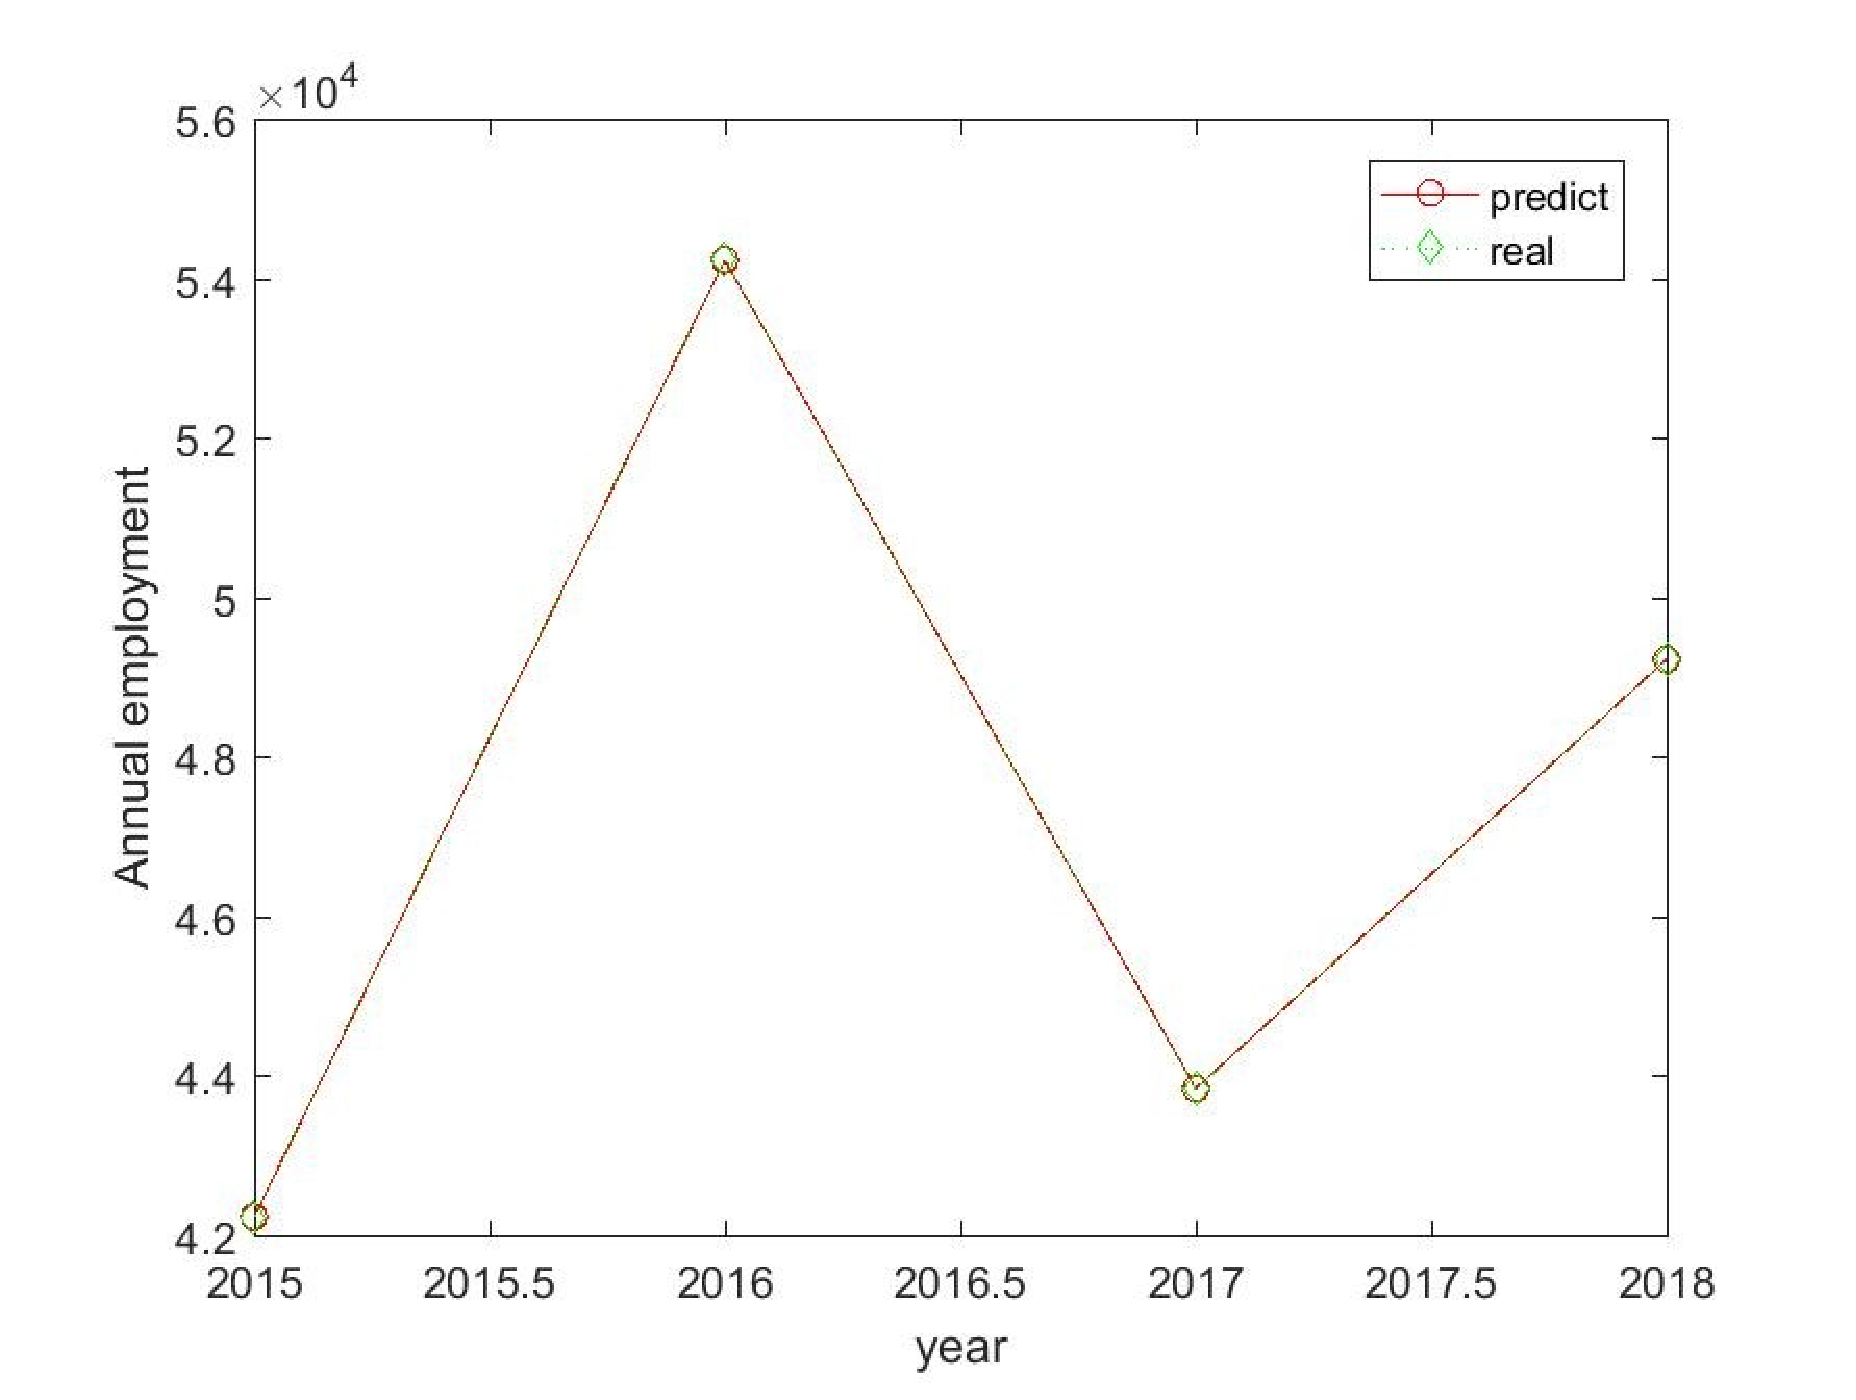
\includegraphics[width=1\textwidth]{2.13.eps}
		\caption{model fitting}
		\label{fig:P2.13}
	\end{minipage}
	\begin{minipage}[h]{0.5\linewidth}
		\centering
		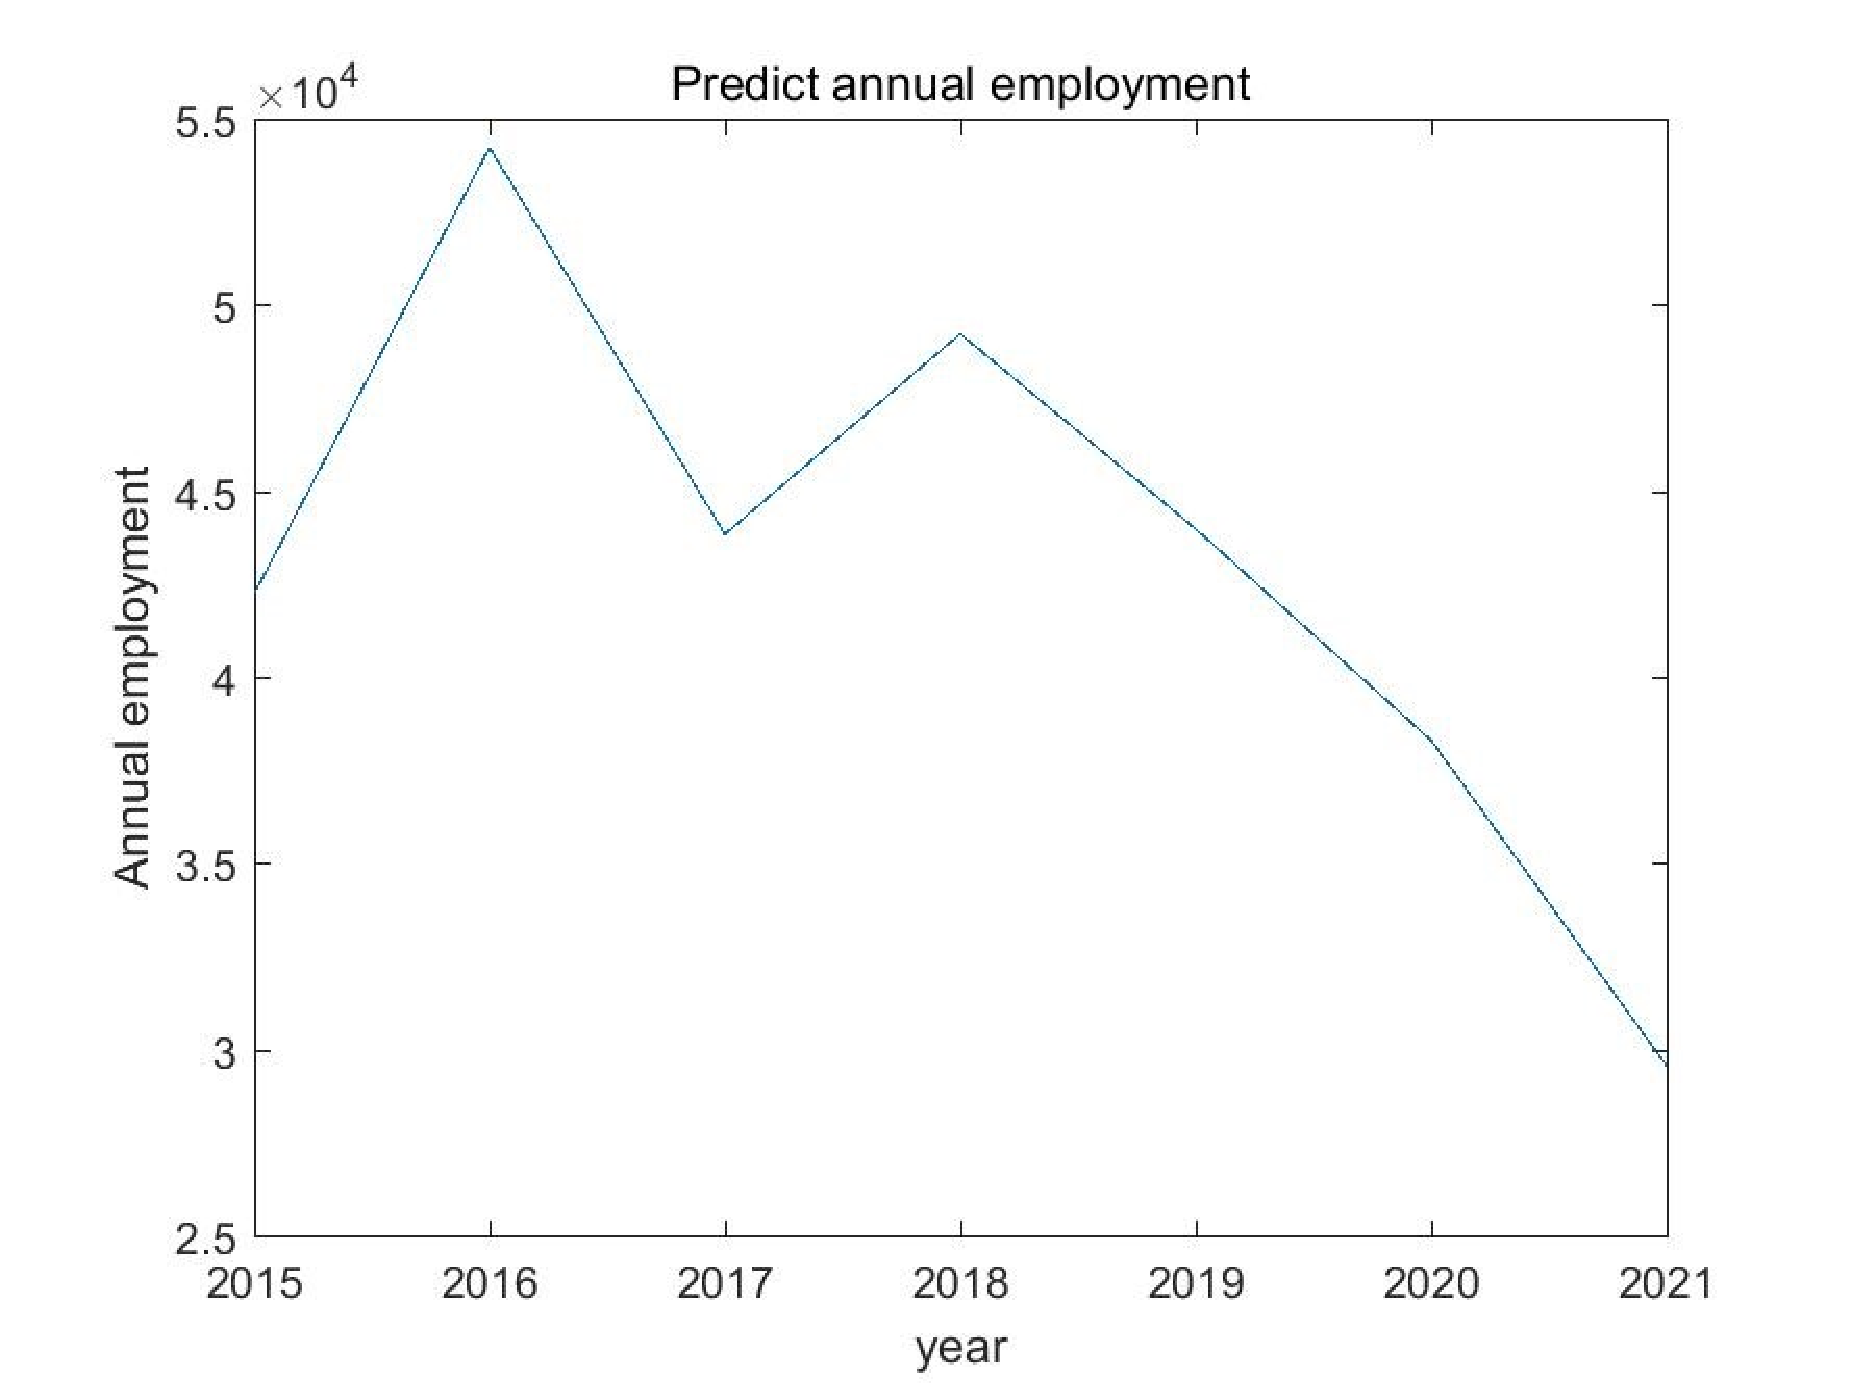
\includegraphics[width=1\textwidth]{2.14.eps}
		\caption{prediction}
		\label{fig:P2.14}
	\end{minipage}
\end{figure}

\subsection{Solution for Problem Three}
\subsubsection{Model Establishment}
 Narrow down the scope of the administrative division of A-city based on Bayesian discriminant method. Bayesian discriminant method can avoid the limitation of linear discriminant method and use Bayesian formula to predict.

\par\noindent
 Firstly, according to the regional development, 28 provinces and municipalities in China are divided into six categories. As shown in the following figure:

\begin{center}
	\begin{tabular}{cc}
		\hline
		\makebox[0.3\textwidth][c]{class}	&  \makebox[0.4\textwidth][c]{city} \\ \hline
		1      & Beijing,Shanghai,Tianjin,Chongqing        \\ \hline
		2	   & Jiangsu,Zhejiang,Shandong,Guangdong		\\ \hline
		3	   & Hebei,Henan,Sichuan      \\ \hline
		4	   & Shanxi,Liaoning,Anhui,Fujian,Jiangxi,Shanxi \\ \hline
		5	   & Neimenggu,Jilin,Heilongjiang,Guangxi,Guizhou,Yunnan \\ \hline
		6      & Hainan,Xizang,Gansu,Qinghai,Ningxia,Xinjiang  \\ \hline
	
	\end{tabular}
\end{center}
Using Naive Bayesian discriminant method, the growth rate of employment is taken as the discriminant basis. For each category, we have the employment growth rate $g_{1,t}$ between 2015 and 2016 and $g_{2,t}$ between 2016-2017. We can easily calculate the employment growth rate $ga_{1,t}$ and $ga_{2,t}$ of A-city from 2015 to 2016 and 2016 to 2017 according to the data of the second question. Then, by screening the features of each category and matching them, A-City can be divided into one of them by using the following Bayesian discriminant algorithm:
\begin{enumerate}
	\item The density functions of six populations G\_1, G\_2,..., G\_6 are $p_1(x),p_2(x),...,p_6(x)$
	\item The prior distributions of six populations G\_1, G\_2,..., G\_6 are $q_1,q_2,...,q_6$
	\item The loss of sample G\_i misjudged as G\_j is c(j | i)
	\item The probability of loss is $p(j|i) = \int\limits_{{D_i}} {{p_i}(x)dx} $
	\item Average loss is $ECM({D_1},{D_2},...,{D_6}) = \sum\limits_{i = 1}^k {{q_i}} \sum\limits_{j = 1}^k {c(j|i)p(j|i)} $, the goal is to make the average loss ECM({D\_1},{D\_2},...,{D\_6}) smallest.
	\item If x falls into D\_i, then x belongs to G\_i
\end{enumerate}
By this way, we can get the general geographical location of A-City.

\subsubsection{Results Analysis}
We use the data of China Statistical Yearbook from 2015 to 2017 and the function classify () of matlab.
\par\noindent
The distance function is chosen as quadratic to solve naive Bayesian discriminant, and the model error is 0.3. A-city belongs to type 1 city. Although the model error is greater than quadratic distance function with other distance functions, the classification results are all 1.
\par\noindent
So we infer that A city may be the first-tier City represented by Beijing, and the administrative division belongs to the municipal level, and the high-tech industry is in the leading level in China.
\par\noindent
The following is a guess of A-city based on Question 2. First of all, the data used in the largest talent market in City A, we can see from the total amount of data, the number of job seekers in the city is huge. In addition, there are a large number of job seekers in the city's high-tech industry - computer software, hardware, finance and so on, indicating that A-city is also among the best in China's high-tech industry. In addition, A-City has more job seekers in the fields of logistics and marketing, and the demand for these positions is also increasing year by year. Through the second question on the demand for talents in A-city in the next few years, in the next few years, the demand for qualifications of talents in the whole market will be higher and higher, which can be more reflected in the computer field. So it can be inferred that A-city high-tech industry is also developing, and should be in the leading position.
\subsection{Solution for Problem Four}
Through targeted searching for career opportunities, we found some data which is stored in the table named ``data\_findOnline\_for\_problem\_four.xlsx" of our supporting materials:
\begin{quote}
\begin{enumerate}
\item Statistics and proportion on graduation directions of three types of students of Tsinghua University in 2017:

\begin{figure}[h]
	%\small
	\centering
	\includegraphics[width=12cm]{Qsinghua.png}
	\caption{Career Selection People Number Comparison in Qsinghua University 2017} \label{fig:P4.2}
\end{figure}

\begin{figure}[h]
	%\small
	\centering
	\includegraphics[width=12cm]{QsinghuaRatio.png}
	\caption{Career Selection Ratio Comparison in Qsinghua University 2017} \label{fig:P4.3}
\end{figure}

\item Statistics about National civil service exam, Graduate examination and oversea-study on the last five years:

\begin{figure}[h]
	%\small
	\centering
	\includegraphics[width=12cm]{exam_oversea.png}
	\caption{Direction Selection -- People Number Comparison} \label{fig:P4.1}
\end{figure}

\item Proportion statistics about the career preferences of China Students on the last five years:
\begin{figure}[h]
	%\small
	\centering
	\includegraphics[width=12cm]{4.png}
	\caption{Career Selection of China Students --  Ratio Comparison } \label{fig:P4.4}
\end{figure}


%\eqref{P4.2}\\
%Figure \ref{P4.2}.
\item Ratio Statistics on Three Graduation Directions of Undergraduates in China:
\begin{figure}[h]
	%\small
	\centering
	\includegraphics[width=12cm]{l.png}
	\caption{Three Graduation Directions Choices of Undergraduates --  Ratio Comparison } \label{fig:P4.5}
\end{figure}

\item Some other data about the person number of various China students.

\par\noindent
\end{enumerate}  
\end{quote}
\noindent
Due to the time limitation and difficulty in finding suitable and complete data, we can't use K-Means algorithm to classify the graduate direction to several different classes which is good for judging trends of career preferences, even more, we have to assign some values for some data accordingly for drawing a complete picture. So in the end we decide to observe the pictures carefully and summarize some conclusions directly and scientifically.\par\noindent
After having some analytical approaches, we obtain the following suggestions:
\begin{quote}
	\begin{enumerate}
		\item Increase the investment of school funds.\par
		Since the sum number of undergraduates、graduates and doctors is increasing year by year which we can see from the pictures above, improving the quality of learning environment and increasing the welfare of universities is a useful way for retaining talents and attracting more talents to enter into and settle down in A-city.
		\item Encourage entrepreneurship, support new enterprises and attract foreign investment.\par
		It's easily to see the proportion of of individuals starting or running their own business is increasing year by year, which contains enormous potential and can inject vigorous vitality into the urban development. As a result, we advise that steps be taken to encourage entrepreneurship and support new enterprises which are mainly from young people, so that the foundations of cities are more solid with the faster economic development. Besides, in order to speed up the development of enterprises, we suggest some favorable policies to attract foreign investment are needed.
		\item Put forward policies to attract overseas returnees.\par
		In respect of the oversea study, we can foresee the increasing number of students aboard must come with the larger number of overseas returnees. Therefore we may reasonably put forward a strategy of overseas talent introduction to A-City.
	\end{enumerate}
	
\end{quote} 
\subsection{Solution for Problem Five}

Data: 2018-11-25  \\

\noindent
Dear school authorities,\\
\\
As students of computer science and finance, we have the following suggestions for schools to cultivate talents:\\
\\
(1) Schools should put students' professional learning and moral cultivation in the first job.\\
\\
(2) Offering minor courses and elective courses to cultivate diversified talents.\\
\\
(3) Carry out innovative and entrepreneurial activities, exercise students' innovative ability. \\
\\
(4) More extracurricular recreational sports activities, improve the overall quality of students.  \\
\\
(5) Cooperate more with computer departments, financial departments and other enterprises to achieve the goal of employment after graduation of talents. \\
\\
The primary task of students is to learn and establish a good moral character, only the moral character of good people can really realize their ideals to make contributions to the society. Therefore, the school should strengthen the school's style of study, set higher graduation assessment standards, and reward students who study well. Secondly, there is an increasing demand for comprehensive talents in the society. It is not enough to master only one specialized knowledge. Therefore, schools should offer more minor courses and elective courses, especially computer major minor courses. More and more jobs require computer knowledge, and the financial sector requires more and more computer knowledge. The current society has changed from element-driven to innovation-driven, which means that only innovation can drive the development of social productivity. Not only does the state encourage creative activities, but schools should pay more attention to students' creative ability. The body is the capital of the revolution, art can edify the soul, only the comprehensive quality of students, in order to better play their ability in the work. If schools can cooperate with enterprises in the market, they can not only provide enterprises with the talents they need, but also increase the employment rate of students, which likes kill two birds with one stone. \\
\\
Best wishes.\\
\\
Yours Sincerely



\section{Model Evaluation}


\subsection{Evaluation for Problem 1}
The model evaluation of the first question: the advantage is that the talent demand is related to the expected occupation, the expected education background and the job demand, and the relationship between the dependent variable and the independent variable can be quantitatively analyzed. And the significance level of each industry can be obtained through fixed effect regression model and dummy variable regression method. However, this model also has some disadvantages. For example, only academic requirements are divided into two groups, resulting in inaccurate results and high assumptions required by the fixed-effect model. In order to improve the model, educational requirements can be further divided into four groups, and more factors can be used to measure the variable talent demand.

\subsection{Evaluation for Problem 2}
The advantage of neural network is that it can predict any function with high precision and automatically process redundant information by reducing weight. However, it is prone to over-fitting and poor interpretation. In this case, the neural network can be used to fit the volatility of the talent market with high accuracy, but the small number of samples may lead to a certain contingency in the fitting.\par
The advantage of grey prediction is that few sample points are needed for prediction. GM(1, 1) models the total number of talents in an exponential form, DGM(2, 1) and GM(2, 1) model the total number of talents in a year by using a second-order differential equation. By using the combined prediction model, the output of the three gray prediction models is weighted sum based on errors, and the final result is obtained. In this way, data with certain volatility can be well fitted. However, the disadvantage is that if the data is highly random, the fitting result is poor. \par
The total employment prediction model is based on student employment situation, regression model and gray prediction can predict the future employment situation of A-city more accurately. However, due to the use of multiple prediction methods, the error is increased to a certain extent. \par
In terms of model improvement, additional statistics can be made on A-city's talent market to obtain more statistical data, and the prediction error can be reduced by increasing the number of statistical data. If the statistics are larger enough, the random forest method can be used to model the change of its talent market. This model can also be applied to the future development statistics of talents in other cities.

\subsection{Evaluation for Problem 3}
Naive bayes test can better judge the category of samples, but in this case, due to the small amount of data, more errors will inevitably be introduced. The accuracy of discrimination can be increased by increasing the amount of data. In this case, however, the model is sufficient because it is only used to narrow the range of possible geographical locations. This model can be improved by statistics and adding more A-city evaluation indexes and evaluation indexes in all regions of the country. It can also predict the geographical range of any other region.

\begin{thebibliography}{99}
\bibitem{1} D.~E. KNUTH   The \TeX{}book  the American
Mathematical Society and Addison-Wesley
Publishing Company , 1984-1986.
\bibitem{2}Lamport, Leslie,  \LaTeX{}: `` A Document Preparation System '',
Addison-Wesley Publishing Company, 1986.
\bibitem{3}\url{http://www.latexstudio.net/}
\bibitem{4}\url{http://www.chinatex.org/}
\bibitem{5} Jeffrey M. wooldridge. Introductory Econometrics.
\bibitem{6} Chen hong. Network traffic prediction model combining autoregressive and neural network.
\bibitem{7} Sun. Mathematical modeling algorithm and application
\bibitem{8} Zhuo. MATLAB mathematical modeling method and practice.
\end{thebibliography}

\begin{appendices}

\section{First appendix}
\appendix

\begin{lstlisting}[language=matlab]
DGM2_1   	grey prediction(2, 1)
GM_month 	grey prediction(1, 1)
GM2_1 		grey prediction(2, 1)
FF2 		BP artificial neural network
main3		qus2_model\_1\_2
main5		qus2_model\_3
main		qus3

function [ err, out, future ] = DGM_2_1( in, len )
%灰度预测GM(2, 1)

A = in;
%A = cumsum(in);             %累加序列作为预测序列
m = length(A);
x0 = A(1 : m - len);        %原始序列
n = length(x0);
x1 = cumsum(x0);            %计算一次累加
z = 0.5 * (x1(2:n) + x1(1:n-1));
B = [-z', z'.^2];
Y = x0(2:end)';
u = B \ Y;  %估计参数a,b的值
syms x(t)
x = dsolve(diff(x)+u(1)*x==u(2)*x^2,...
x(0)==x0(1));  %求符号解
xt = vpa(x, 6);  %显示小数形式的符号解
yuce = subs(x, 't', 0:n-1);    %求已知数据点1次累加序列的预测值
yuce = double(yuce);
x0_hat = [yuce(1), diff(yuce)];  %求已知序列的预测值
epsilon = x0 - x0_hat;           %求残差
delta = abs(epsilon ./ x0);      %求相对残差
[x0_hat' A(1:m-len)']

err = x0_hat - A;
out = x0_hat;
future1 = subs(x, 't', length(A):length(A)+2);
future1 = double(future1);
future = [future1(1), diff(future1)];

%{
out1 = subs(x, 't', n:n+len-1);
out1 = double(out1);
out = [out1(1), diff(out1)];

err = out - A(m-len+1:m);

future1 = subs(x, 't', n+len:n+len+11);
future1 = double(future1);
future = [future1(1), diff(future1)];

[x0_hat' A(1:m-len)']
figure
plot(1:m-len, x0_hat, 'o-r');
hold on
plot(1:m-len, A(1:m-len), 'd--g');
legend('预测值', '真实值');
close
%}

function [err, out, future] = FF2(inputs)
%自回归神经网络

lag = 3;    %自回归的阶数
ep = 5;
input = inputs(1 : size(inputs, 2)-ep);
test = inputs(size(inputs, 2)-ep+1 : size(inputs, 2));
T = input(lag + 1 : size(input, 2));  %target
P = zeros(lag, size(input, 2) - lag);
for i = 1 : size(input, 2) - lag
P(:, i) = input(i:i+lag-1)';
end  %input
net = newff(P, T, [35 25 15], {'logsig' 'tansig' 'purelin'}, 'traingd',...
'learngd', 'sse');      %建立一个前馈反向神经网络 
me = 16000;
%划分训练集
%{
net.divideParam.trainRatio = 70/100;
net.divideParam.valRatio = 15/100;
net.divideParam.testRatio = 15/100;
%}
net.trainParam.show = 10;    %两次之间的训练次数
net.trainParam.goal = 0.01; %目标误差
net.trainParam.lr = 0.01;    %网络的学习速率
net.trainFcn = 'traingda';    %变学习率梯度下降算法
A = sim(net, P);             %训练前的网络输出
sse = sum(abs(A - T) ./ T) / size(T, 2);         %训练的均方误差
for i = 1 : me / 100
if sse < 0.1     %神经网络停止条件
i = i - 1;
break;
end
net.trainParam.epochs = 100;    %最大训练次数
[net, tr] = train(net, P, T);   %训练神经网络
trp( (1+100*(i-1)):(max(tr.epoch)+...
100*(i-1)) ) = tr.perf(1:max(tr.epoch));
A = sim(net, P);
sse = sum(abs(A - T) ./ T) / size(T, 2);
sse
end
%{
figure
plot(trp);
[i, j] = size(trp);
hold on
plot(1:j, net.trainParam.goal, 'r--');
hold off
title('Error Signal');
xlabel('epoch');
ylabel('Error');
%}
%{
y = net(P);
errors = T - y;
figure, ploterrcorr(errors) %误差自相关
figure, parcorr(errors)     %误差偏相关
figure, plotresponse(con2seq(T), con2seq(y));
%预测趋势与原趋势
figure, ploterrhist(errors) %误差直方图
figure, plotperform(tr)     %误差下降线
%}

y = net(P);
figure
plot(1:size(P, 2), y, 'o-g');
hold on
plot(1:size(P, 2), T, 'd:r');
legend('predicted value', 'real value');

in = input(size(input, 2) - lag + 1 : size(input, 2))';
out = zeros(1, ep);
for i = 1 : ep
out(i) = net(in);
in = [in(2:lag); out(i)];
end
figure
plot(1:ep, out, '-or');
hold on
plot(1:ep, test, '--dg');
legend('predicted value', 'real value');
title('talent demand forcast');
xlabel('days');
ylabel('talent demad');

err = out - test;

%预测未来三年
ep2 = 41;
in = input(size(input, 2) - lag + 1 : size(input, 2))';
out2 = zeros(1, ep2);
for i = 1 : ep
out2(i) = net(in);
in = [in(2:lag); out(i)];
end
future = out2(6 : 41);

function [ err, out, future ] = GM_2_1( in, len )
%灰度预测GM(2, 1)
A = in;
%A = cumsum(in);             %累加序列作为预测序列
m = length(A);
x0 = A(1 : m - len);        %原始序列
n = length(x0);
x1 = cumsum(x0);            %计算一次累加
a_x0 = diff(x0)';           %计算1次累减
z = 0.5 * (x1(2:end)+x1(1:end-1))'; %计算均值生成函数
B = [-x0(2:end)', -z, ones(n-1, 1)];
u = B \ a_x0;               %最小二乘法拟合参数
syms x(t)
x = dsolve(diff(x, 2) + u(1) * diff(x) + u(2) * x == u(3), ...
x(0) == x1(1), x(3) == x1(4));  %求符号解
xt = vpa(x, 6);             %显示小数形式的符号解
yuce = subs(x, t, 0 : n-1); %求已知数据点1次累加序列的预测值
yuce = double(yuce)         %符号数转换为数值类型,否则无法做差分运算
x0_hat = [yuce(1), diff(yuce)];
x0_hat = round(x0_hat)      %四舍五入取整数

%输出
err = x0_hat - A;
out = x0_hat;
future1 = subs(x, 't', length(A):length(A)+2);
future1 = double(future1);
future = [future1(1), diff(future1)];
%{
x0_len = length(x0_hat);
res(2:x0_len) = x0_hat(2:x0_len) - x0_hat(1:x0_len-1);
res(1) = A(1);
%}
%{
out1 = subs(x, 't', n:n+len-1);
out1 = double(out1);
out = [out1(1), diff(out1)];

err = out - A(m-len+1:m);

future1 = subs(x, 't', n+len:n+len+11);
future1 = double(future1);
future = [future1(1), diff(future1)];

[x0_hat' A(1:m-len)']
figure
plot(1:m-len, x0_hat, 'o-r');
hold on
plot(1:m-len, A(1:m-len), 'd--g');
close
epsilon = x0 - x0_hat       %求残差
delta = abs(epsilon ./ x0)  %求相对误差
%}

function [ err, out, future ] = GM_month( As, name, x )
%灰度预测GM(1, 1)

m = size(As, 2);
A = As(1: m-x);
syms a b;
c = [a b]';
B = cumsum(A);        %B为A的累加
n = length(A);
for i = 1 : n - 1     %C为B的紧邻均值
C(i) = (B(i) + B(i+1)) / 2;
end

%计算待定参数的值
D = A;
D(1) = [];
D = D';
E = [-C; ones(1, n-1)];

%用最小二乘法求出a,b的值
c = inv(E * E') * E * D;
c = c';
a = c(1);
b = c(2);

%预测后续数据
F = [];
F(1) = A(1);
for i = 2 : n + x
F(i) = (A(1) - b / a) / exp(a * (i - 1)) + b / a;
end

G = [];
G(1) = A(1);
for i = 2 : n + x
G(i) = F(i) - F(i-1);
end
t1 = 1:n;
t2 = 1:n+x;
G

err = G(1:m) - As(1:m);
out = G(1:m);
%{
figure
plot(t2, As, 'o', t2, G);
out = G(m-x+1:m);
hold on
xlabel('time');
ylabel(['position number of' name]);
title(name);
%saveas(gca, ['total_demand/' name '.jpg'])
close
%}

%预测未来三年数据
F = [];
F(1) = A(1);
for i = 2 : n + x + 12
F(i) = (A(1) - b / a) / exp(a * (i - 1)) + b / a;
end

G = [];
G(1) = A(1);
for i = 2 : n + x + 3
G(i) = F(i) - F(i-1);
end
future = G(n+x+1:n+x+3);

clc

[~, ~, data_in] = xlsread('CH0407.xls');
[~, ~, data_in_2] = xlsread('CH0407_2.xls');
[~, ~, data_in_3] = xlsread('CH0407_3.xls');
flag = [1
1
3
4
5
4
5
5
1
2
2
4
4
4
2
3
3
3
2
5
6
1
3
5
5
6
4
6
6
6
6
];

data = data_in(10:size(data_in, 1), 3:size(data_in, 2));        %16年数据
data2 = data_in_2(8:size(data_in_2, 1), 3:size(data_in_2, 2));  %17年数据
data3s = data_in_3(9:size(data_in_3, 1), 5:size(data_in_3, 2));
data = cell2mat(data);
data2 = cell2mat(data2);
for i = 1 : size(data3s, 1)
for j = 1 : size(data3s, 2)
data3(i, j) = str2double(data3s{i, j});
end
end
%%
%分行业增长率
[height, width] = size(data); 
growth_rate_1 = (data2(1:height, 2:width) - ...
data(1:height, 2:width)) ./ data(1:height, 2:width);  
%16~17 增长率
growth_rate_2 = (data(1:height, 2:width) - ...
data3(1:height, 2:width)) ./ data3(1:height, 2:width);  
%15~16 增长率

%%
%总增长率
tot_data_1 = zeros(1, height);  %17
tot_data_2 = zeros(1, height);  %16
tot_data_3 = zeros(1, height);  %15
growth_tot_1 = zeros(1, height);    %16~17增长率
growth_tot_2 = zeros(1, height);    %15~16增长率
for i = 1 : height
tot_data_1(i) = sum(data(i, :));
tot_data_2(i) = sum(data2(i, :));
tot_data_3(i) = sum(data3(i, :));
end
growth_tot_1 = (tot_data_1 - tot_data_2) ./ tot_data_2;
growth_tot_2 = (tot_data_2 - tot_data_3) ./ tot_data_2;

[~, ~, res] = xlsread('数据1.xls');
[~, index] = sort(res(:, 13));
res2 = res(index, :);
bg = 1;
sum_ppl = zeros(1, 4);
tot_ppl = zeros(1, 4);
for i = 2 : size(res2, 2)
tt = res{i, 13};
yy = str2double(tt(1:4));
for j = 4 : 12
sum_ppl(yy-2014) = sum_ppl(yy-2014) + res{i, j};
end
tot_ppl(yy-2014) = tot_ppl(yy-2014) + 1;
end
sum_ppl = sum_ppl ./ tot_ppl;
training = [growth_tot_1', growth_tot_2'];
group = flag';
sample = [(sum_ppl(3)-sum_ppl(2))/sum_ppl(2),...
(sum_ppl(2)-sum_ppl(1))/sum_ppl(1)];
[class, err] = classify(sample, training, group, 'quadratic');

clc

[~, ~, res] = xlsread('数据1.xls');
[~, ~, res3] = xlsread('2011.01.01-2012.12.14.xls');
guokap = [140.9, 139.46, 148.63, 165.97];
biye = [749, 756, 795, 820];
data_cha = [140.9  140.9 139.46 139.46 139.46 139.46 ...
148.63 148.63 148.63 148.63 ...
165.97 165.97 165.97;
749 749 756 756 756 756 795 795 795 795 ...
820 820 820];
beg = 1;
name = 1;
data = [];
[~, index] = sort(res(:, 13));

res2 = res(index, :);
w = [1 2 3 4 5 6 7 8 1];
w = w / sum(w);
for i = 2 : size(res, 1)
if strcmp(res(i, 2), res(i - 1, 2)) == 0
ed = i - 1;
tot = 0;
sumpeo = zeros(1, 13);
tot = zeros(1, 13);
y_sum = zeros(1, 4);
y_tot = zeros(1, 4);
for j = beg : ed
tt = res{j, 13};
yy = str2double(tt(1:4));
mm = str2double(tt(6));
if strcmp(tt(8), '/') == 1
mm2 = str2double(tt(7));
mm = mm * 10 + mm2;
end
%yy为年份
%mm为月份

cal = res{j, 6} + res{j, 7} + res{j, 8};
if yy == 2015
y_sum(1) = y_sum(1) + cal;
y_tot(1) = y_tot(1) + 1;
if mm == 9
sumpeo(1) = sumpeo(1) + ...
cal;
tot(1) = tot(1) + 1;
end
if mm >= 10 && mm <= 12
sumpeo(2) = sumpeo(2) + ...
cal;
tot(2) = tot(2) + 1;
end
end
if yy == 2016
y_sum(2) = y_sum(2) + cal;
y_tot(2) = y_tot(2) + 1;
if mm >= 1 && mm <= 3
sumpeo(3) = sumpeo(3) + ...
cal;
tot(3) = tot(3) + 1;
end
if mm >= 4 && mm <= 6
sumpeo(4) = sumpeo(4) + ...
cal;
tot(4) = tot(4) + 1;
end
if mm >= 7 && mm <= 9
sumpeo(5) = sumpeo(5) + ...
cal;
tot(5) = tot(5) + 1;
end
if mm >= 10 && mm <= 12
sumpeo(6) = sumpeo(6) + ...
cal;
tot(6) = tot(6) + 1;
end
end
if yy == 2017
y_sum(3) = y_sum(3) + cal;
y_tot(3) = y_tot(3) + 1;
if mm >= 1 && mm <= 3
sumpeo(7) = sumpeo(7) + ...
cal;
tot(7) = tot(7) + 1;
end
if mm >= 4 && mm <= 6
sumpeo(8) = sumpeo(8) + ...
cal;
tot(8) = tot(8) + 1;
end
if mm >= 7 && mm <= 9
sumpeo(9) = sumpeo(9) + ...
cal;
tot(9) = tot(9) + 1;
end
if mm >= 10 && mm <= 12
sumpeo(10) = sumpeo(10) + ...
cal;
tot(10) = tot(10) + 1;
end
end
if yy == 2018
y_sum(4) = y_sum(4) + cal;
y_tot(4) = y_tot(4) + 1;
if mm >= 1 && mm <= 3
sumpeo(11) = sumpeo(11) + ...
cal;
tot(11) = tot(11) + 1;
end
if mm >= 4 && mm <= 6
sumpeo(12) = sumpeo(12) + ...
cal;
tot(12) = tot(12) + 1;
end
if mm >= 7 && mm <= 9
sumpeo(13) = sumpeo(13) + ...
cal;
tot(13) = tot(13) + 1;
end
end
end
sumpeo_len = length(sumpeo);
data = sumpeo ./ tot;
for j = 1 : sumpeo_len
if tot(j) == 0
data(j) = 0;
end
end
data2 = y_sum ./ y_tot;
err = zeros(3, 4);
out = zeros(3, 4);
future = zeros(3, 3);
[err_bp, out_bp, future_bp] = FF(data);
[err(1, :), out(1, :), future(1, :)] = DGA_2_1(data2, 0);
[err(2, :), out(2, :), future(2, :)] = GM_2_1(data2, 0);
[err(3, :), out(3, :), future(3, :)] = GM_month(data2, [res{beg, 2} ' ' num2str(1)], 0);
beg = i;
%{
D(1) = 1 / sum(err1.^2);
D(2) = 1 / sum(err2.^2);
D(3) = 1 / sum(err3.^2);
D(4) = 1 / sum(err4.^2);
%}
D(1) = 1 / sum(err(1,:) .^ 2);
D(2) = 1 / sum(err(2,:) .^ 2);
D(3) = 1 / sum(err(3,:) .^ 2);
k = D / sum(D);
out = round(k * out);
len = length(data);
%{
figure
plot(1:2, data(len-1:len), '-or');
hold on
plot(1:2, out, '--dg');
title([res{beg, 2} ' ' num2str(1)]);
xlabel('season');
ylabel('talent demand');
legend('true value', 'predict value');
%}
future_e = k * future;
bri = res{beg, 2};
figure
plot(2019:2021, future_e, '-o');
title(['future prediction' res{beg, 2} ' ' num2str(1)]);
saveas(gca, ['预测数据2/' bri(1:min(length(bri), 3)) '(1~3).jpg']);
close
xlswrite(['预测数据2/数据预测值(4~6)/' bri(1:min(length(bri), 3)) '(1~3).xls'], [future_e';-1; future_bp']);
figure
plot(1:12, future_bp, '-o');
title(['future prediction of artificial network' res{beg, 2} ' ' num2str(1)]);
saveas(gca, ['预测数据2/' bri(1:min(length(bri), 3)) '(1~3 BP).jpg']);
close
end
end

clc

[~, ~, res] = xlsread('数据1.xls');
[~, index] = sort(res(:, 13));
res2 = res(index, :);
bg = 1;
sum_ppl = zeros(1, 4);
tot_ppl = [4 12 12 8];

for i = 1 : size(res2, 1)
tt = res2{i, 13};
yy = str2double(tt(1:4));
for j = 4 : 12
sum_ppl(yy-2014) = sum_ppl(yy-2014) + res2{i, j};
end
end
sum_ppl = sum_ppl ./ tot_ppl;       %行业的总人口数

%{
高校毕业生初次就业人数(万人)
高校同届招生人数(万人)
国内生产总值(亿元)
年末城镇总人口数(万人)
年末乡村总人口数(万人)
全国人口自然增长率(%)
%}

stu14 = [
527.49
661.76
643974.00
74916.00
61866.00
0.52];

stu15 = [
544.71
681.50
689052.10
77116.00
60346.00
0.50
];

stu16 = [  
563.34
688.83
743585.50
79298.00
58973.00
0.59
];

stu17 = [
795
690
827122
81347
57661
0.59
];

stu18 = [
820
694
867852
83000
56500
0.57
];

figure
for i = 1 : 6
plot(2015:2018, [stu15(i) stu16(i) ...
stu17(i) stu18(i)]);
hold on
end
legend('1', '2', '3', '4', '5', '6');
title('Employment situation of college students and some national conditions of China');
saveas(gca, '大学生就业情况统计图.jpg');
close

stu = [stu15 stu16 stu17 stu18]';
Y = sum_ppl';
X = stu;
[b, bint, r, rint, s] = regress(Y, X);
out1 = b' * stu15;
out2 = b' * stu16;
out3 = b' * stu17;
out4 = b' * stu18;
plot(2015:2018, 12 * [out1 out2 out3 out4], 'or-');
hold on
plot(2015:2018, 12 * sum_ppl, 'dg:');
legend('predict', 'real');
xlabel('year');
ylabel('Annual employment');
saveas(gca, '预测结果图.jpg');
close
future = zeros(6, 3);
for i = 1 : 6
[~, ~, future(i, :)] = GM_month([stu15(i) stu16(i) stu17(i) stu18(i)], '', 0);
end
out = b' * future;
plot(2015:2021, 12 * [sum_ppl, out]);
title('Predict annual employment');
xlabel('year');
ylabel('Annual employment');
saveas(gca, '预测就业人口总数结果图.jpg');
close
%{
回归系数

-19.0794
0
0.0709
-0.8401
0.4944
0

预测总岗位数
1.0e+04 *

4.2231
5.4229
4.3837
4.9221
4.3977
3.8294
2.9549
%}



\end{lstlisting}
\end{appendices}
\end{document}

%%
%% This work consists of these files mcmthesis.dtx,
%%                                   figures/ and
%%                                   code/,
%% and the derived files             mcmthesis.cls,
%%                                   mcmthesis-demo.tex,
%%                                   README,
%%                                   LICENSE,
%%                                   mcmthesis.pdf and
%%                                   mcmthesis-demo.pdf.
%%
%% End of file `mcmthesis-demo.tex'.
